\documentclass[final,3p,times,twocolumn]{elsarticle}

%% The numcompress package shorten the last page in references.
%% `nodots' option removes dots from firstnames in references.
\usepackage[nodots]{numcompress}

%% The lineno packages adds line numbers. Start line numbering with
%% \begin{linenumbers}, end it with \end{linenumbers}. Or switch it on
%% for the whole article with \linenumbers after \end{frontmatter}.
\usepackage{lineno}

%% Avoids linenumbers to collide with text for 5p format:
\setlength\linenumbersep{3pt}

%\usepackage{amsmath,amsthm,amsfonts,amscd,amssymb,amstext} 
\usepackage{amsmath,amsfonts,amscd,amssymb,amstext} 
\usepackage{mathrsfs}
				% Some packages to write mathematics.
\usepackage{overpic}
\usepackage{eucal} 	 	% Euler fonts
\usepackage{verbatim}      	% Allows quoting source with commands.
\usepackage{makeidx}       	% Package to make an index.
%\usepackage{citesort}         	% 
\usepackage{subfig}
\usepackage{graphicx}
\usepackage{url}		% Allows good typesetting of web URLs.
\usepackage{multirow}
%\usepackage[linesnumbered, noline]{algorithm2e}
%\usepackage[boxed, noline]{algorithm2e}
\usepackage[ruled]{algorithm2e}
\usepackage{booktabs}
\usepackage{tabularx}
\usepackage{array}
\usepackage{adjustbox}
\usepackage{color}
\usepackage{tikz}
% To balance the columns at the end
\usepackage{balance}
\usepackage[mediumspace,mediumqspace,Grey,squaren]{SIunits}
%\usepackage{draftcopy}		% Uncomment this line to have the
				% word, "DRAFT," as a background
				% "watermark" on all of the pages of
				% of your draft versions. When ready
				% to generate your final copy, re-comment
				% it out with a percent sign to remove
				% the word draft before you re-run
				% Makediss for the last time.
\usepackage[normalem]{ulem}

%\usepackage{cite}
\usepackage{balance}
\usepackage{color}

\definecolor{bostonuniversityred}{rgb}{0.8, 0.0, 0.0}
\definecolor{medblue}{rgb}{0.0, 0.0, 0.7}

%------------------------------------------------------------
% Custom commands
%------------------------------------------------------------
%\newcommand{\old}[1]{\textcolor{blue}{\sout{#1}}}
\newcommand{\old}[1]{}

%\newcommand{\red}[1]{\textcolor{red}{#1}}
\newcommand{\red}[1]{\textcolor{bostonuniversityred}{#1}}
\newcommand{\blue}[1]{\textcolor{medblue}{#1}}
\definecolor{light-gray}{gray}{0.75}
\newcommand{\gray}[1]{\textcolor{light-gray}{#1}}
%\newcommand{\red}[1]{#1}

%\newcommand{\reconstruct}{RECONSTRUCT\textsuperscript{\texttrademark}}
%\newcommand{\tm}{\textsuperscript{\texttrademark}}
\newcommand{\tm}{$^1$}
\newcommand{\addref}{\red{REF}}
\newcommand{\mathtext}[1]{\text{#1}}
\newcommand{\etal}{et al.\ }
\newcommand{\algorithmspace}{\vspace{8pt}}
\newcommand{\glfs}{\emph{glfs}}

\renewcommand{\vec}[1]{\mathbf{#1}}

\newcommand{\centercell}[1]{\multicolumn{1}{c}{#1}}
\newcolumntype{x}[1]{>{\centering\arraybackslash\hspace{0pt}}m{#1}}
\newcolumntype{y}[1]{>{\centering\arraybackslash\hspace{0pt}}m{#1\textwidth}}
\newcolumntype{M}{>{\centering\arraybackslash}m{1cm}}

\DeclareMathOperator*{\argmin}{arg\,min}
\DeclareMathOperator*{\argmax}{arg\,max}

\newcommand{\BigO}[1]{\ensuremath{\operatorname{O}\left(#1\right)}}
\newcommand{\centroid}{\mathscr{C}}
\newcommand{\iring}{\mathscr{R}}

% aligned
\renewcommand{\d}{\delta}
\newcommand{\vempty}{\mathscr{E}}
\newcommand{\e}{\epsilon}
\newcommand{\dist}{\mathtext{dist}}
\newcommand{\ball}{\mathscr{B}}


\newcommand{\hgt}{22mm}

%%--------------------------------------------------
%% Theorem environments (amsthm package required)
%%--------------------------------------------------
%% \theoremstyle{plain} %% This is the default
%\newtheorem{theorem}{Theorem}
%\newtheorem{lemma}{Lemma}
%\newtheorem{corollary}{Corollary}
%\newtheorem{conjecture}{Conjecture}
%\newtheorem{crit}{Criterion}
%\newtheorem{condition}{Condition}
%\newtheorem{fact}{Fact}

%\theoremstyle{definition}
%\newtheorem{defn}{Definition}[section]

%\theoremstyle{remark}
%\newtheorem{rem}{Remark}[section]
%\newtheorem*{notation}{Notation}

%\numberwithin{equation}{section}

%--------------------------------------------------
% Tight enumerations
%--------------------------------------------------
\newenvironment{tightenumerate}{
\begin{enumerate}
  \setlength{\itemsep}{1pt}
  \setlength{\parskip}{0pt}
  \setlength{\parsep}{0pt}
}{\end{enumerate}
}
\newenvironment{tightitemize}{
\begin{itemize}
  \setlength{\itemsep}{1pt}
  \setlength{\parskip}{0pt}
  \setlength{\parsep}{0pt}
}{\end{itemize}
}

%--------------------------------------------------
% Add figs to graphics path
%--------------------------------------------------
\graphicspath{{./}{./figs/}}

\newcolumntype{H}{@{}>{\lrbox0}l<{\endlrbox}}

%\newcommand{\container}[2]{container(#1, #2)}
\newcommand{\container}[1]{container(#1)}

\newcommand{\directAncestors}[1]{direct\_ancestors(#1)}

\newcommand{\lcp}{\textit{lcp}}

\newcommand{\shortcite}[1]{\cite{#1}}

\renewcommand{\paragraph}[1]{\noindent \textbf{#1}}



%-------------------------------------------------------------------------
\begin{document}

\begin{frontmatter}

%% Title, authors and addresses

%% use the tnoteref command within \title for footnotes;
%% use the tnotetext command for the associated footnote;
%% use the fnref command within \author or \address for footnotes;
%% use the fntext command for the associated footnote;
%% use the corref command within \author for corresponding author footnotes;
%% use the cortext command for the associated footnote;
%% use the ead command for the email address,
%% and the form \ead[url] for the home page:
%%
%% \title{Title\tnoteref{label1}}
%% \tnotetext[label1]{}
%% \author{Name\corref{cor1}\fnref{label2}}
%% \ead{email address}
%% \ead[url]{home page}
%% \fntext[label2]{}
%% \cortext[cor1]{}
%% \address{Address\fnref{label3}}
%% \fntext[label3]{}

%\title{Parallel Quadtree Construction on Collections of Objects}
\title{Fast Construction of Inter-Object Space Representations}

%\author{Nathan Morrical}
%\author{John Edwards}
%\address{Department of Informatics and Computer Science, Idaho State University, USA}

%% use optional labels to link authors explicitly to addresses:
%% \author[label1,label2]{<author name>}
%% \address[label1]{<address>}
%% \address[label2]{<address>}


%\teaser{
%  \subfloat[][]{
%    \label{fig:gears1}
%    \begin{tikzpicture}
%      \node[anchor=south west,inner sep=0] at (0,0) {
%        \begin{tabular}[b]{c}
%          \includegraphics[height=0.8in]{gears-far1.png} \\
%          \includegraphics[height=0.8in]{gears-close1.png}
%        \end{tabular}
%      };
%      \draw[black,thick] (1.4,3.2) rectangle (2.0,3.6);
%      \draw[black,dashed] (1.4,3.6) -- (0.22,2.15);
%      \draw[black,dashed] (2.0,3.6) -- (2.95,2.15);
%      \draw[black,thick] (0.22,0.1) rectangle (2.95,2.15);
%    \end{tikzpicture}
%  }
%  \subfloat[][]{
%    \label{fig:gears}
%    \begin{tikzpicture}
%      \node[anchor=south west,inner sep=0] at (0,0) {
%        \begin{tabular}[b]{c}
%          \includegraphics[height=0.8in]{gears-far4.png} \\
%          \includegraphics[height=0.8in]{gears-close4.png}
%        \end{tabular}
%      };
%      \draw[black,thick] (1.3,3.1) rectangle (1.9,3.5);
%      \draw[black,dashed] (1.3,3.5) -- (0.22,2.15);
%      \draw[black,dashed] (1.9,3.5) -- (2.92,2.15);
%      \draw[black,thick] (0.22,0.1) rectangle (2.92,2.15);
%    \end{tikzpicture}
%  }
%  \hspace{3mm}
%  \subfloat[][]{
%    \label{fig:knife}
%    \includegraphics[trim=4cm 0cm 4cm 2.5cm, clip=true, height=1.4in]
%                    {knife-above/slice-00000.png}
%  }
%  \subfloat[][]{
%    \label{fig:knife2}
%    \includegraphics[trim=2mm 0cm 2mm 2cm, clip=true, height=1.4in]
%                    {knife-above/slice-00110.png}
%  }
%  \caption{Two example applications of the \red{approximated} generalized Voronoi diagram (GVD) computed by our novel, adaptive algorithm. Previous GVD methods require a gridded space of $2^{24}$ (gears dataset) and $2^{36}$ (knives dataset) voxels to resolve the closely spaced objects.
%    \protect\subref{fig:gears1} Two gears with regions of very tight spacing.
%    \protect\subref{fig:gears} The GVD of the gears model.  The surface is colored red in areas of very close tolerance.
%    \protect\subref{fig:knife} Three butter knives in a wood block.  To animate removal of the knives without intersecting the block requires extreme care because of close mesh spacing.
%    \protect\subref{fig:knife2} Intersection-free motion is guaranteed by computing motion vectors based on the GVD and allowing motion only within a Voronoi cell.
%  }
%  \label{fig:teaser}
%}
%
%\maketitle

\begin{abstract}
We present a parallel quadtree algorithm that resolves between geometric objects, modeling space between objects rather than the objects themselves. Our quadtree has the property that no cell intersects more than one labeled object. A popular technique for discretizing space is to impose a uniform grid -- an approach that is easily parallelizable but often fails because object separation isn't known a priori or because the number of cells required to resolve closely spaced objects exceeds available memory. Previous parallel algorithms that are spatially adaptive, discretizing finely only where needed, \red{Hierarchical kernel envokation isn't necessarily bad. We might move to that to remove some of the Q linear complexity overhead.} either separate points only, or make no guarantees of object separation. Our 2D algorithm is the first to construct an object-resolving discretization that is hierarchical (saving memory) yet with a fully parallel approach (saving time). We describe our algorithm, derive the time complexity, demonstrate experimental results, and discuss extension to 3D. Our results show significant improvement over the current state of the art.

%   Leave one blank line after the abstract, 
%   then add the subject categories according to the ACM Classification Index 
%   (see http://www.acm.org/class/1998/).

%\begin{classification} % according to http://www.acm.org/class/1998/
%  \CCScat{I.3.5}{Computer Graphics}{Computational Geometry and Object Modeling}{Boundary representations}
%  \CCScat{I.3.6}{Computer Graphics}{Methodology and Techniques}{Graphics data structures and data types}
%  %\CCScat{Computer Graphics}{I.3.3}{Picture/Image Generation}{Line and curve generation}
%\end{classification}

\end{abstract}

\end{frontmatter}

%%
%% Start line numbering here if you want
%%
\linenumbers

%-------------------------------------------------------------------------
% Body
%-------------------------------------------------------------------------

%-------------------------------------------------------------------------------
% introduction
%-------------------------------------------------------------------------------
\section{Introduction}
\label{sec:intro}
Constructing quadtrees on objects is an important task with applications in collision detection, distance fields, robot navigation, shape modeling, object description, and other applications. Quadtrees built on objects most often model the objects themselves, providing a space-efficient representation of arbitrarily complex objects. However, our work centers on using quadtrees to separate, or resolve, collections of closely spaced objects, i.e., to construct a discretization such that no cell intersects more than one object. Such quadtrees can be thought of as modeling the space between objects.
% Our quadtree representation is not purposed for fast retrieval as is often the case in hierarchical subdivisions of point data.
% Rather, the quadtrees are used for constructing distance fields, detecting collisions and computing the GVD \cite{edwards2015approximating}.

Modeling inter-object spacing is computationally straightforward when the spacing is large compared to the world bounding box. Approaches typically involve a uniform grid of the space, which leads to efficient computation that often uses graphics processors.

Difficulties arise when objects are close together relative to the size of the domain. An approach using a uniform grid would have excessive memory requirements in order to resolve between objects because the uniformly sized grid cell must be small enough to fit between objects at every location in the domain. Thus, an adaptive approach must be used for datasets of closely spaced objects.

To our knowledge, only one algorithm \cite{edwards2015approximating} computes an adaptive data structure that fully resolves between objects without using unreasonable amounts of memory, but it does so in serial, with expected performance liabilities. A naive approach to parallelizing quadtree computation would be to assign all available compute units according to a course grid, then run the serial algorithm on each compute unit. While simple, there is potential for serious load imbalancing if the close object spacings are not uniformly distributed.

To our knowledge, only one algorithm \cite{edwards2015approximating} computes an adaptive data structure that fully resolves between objects without using unreasonable amounts of memory, but it does so in serial, with expected performance liabilities. A naive approach to parallelizing quadtree computation would be to assign all available compute units according to a course grid, then run the serial algorithm on each compute unit. While simple, there is potential for serious load imbalancing if the close object spacings are not uniformly distributed.

This paper extends the work done by Edwards \etal \cite{edwards2015approximating} by computing the quadtree in parallel with an algorithm that is adaptive and independent of object distribution. Our algorithm, which is targeted for the GPU, performs an order of magnitude faster than the previous work and will be an important base for later distance transform and generalized Voronoi diagram computation.

Our algorithm has three main components:

\begin{enumerate}
\item Construct a quadtree on object vertices using the Karras algorithm \cite{karras2012maximizing}
\item Detect quadtree cells that intersect more than one object, which we call ``conflict cells'' (contribution)
\item Subdivide conflict cells to resolve objects (contribution)
\end{enumerate}

Each step is done in parallel either on object vertices, object facets, or quadtree cells.

Modeling object separation is of some use in 2D (e.g. path planning), but it is a very important problem in many 3D applications. Hierarchically subdividing space between faceted objects in a principled parallel way is complex, and this paper lays the groundwork for our continuing efforts in 3D.

%-------------------------------------------------------------------------------
% Related work
%-------------------------------------------------------------------------------
\section{Related work}

\paragraph{Serial} In an early work, Lavender \etal \shortcite{lavender1992voronoi} define and compute octrees over a set of solid models. 
% JME: note that in the Bastos work, ``reconstruction'' is reconstruction
% of the surface from the quadtree at rendering time.
Two seminal works build octrees on objects in order to compute the Adaptive Distance Field (ADF) on octree vertices.  Strain \shortcite{strain1999fast} fully resolves the quadtree everywhere on the object surface, and Frisken \etal \shortcite{frisken2000adaptively} resolve the quadtree fully only in areas of small local feature size.  Both approaches are designed to retain features of a single object rather than resolving between multiple objects, as is required for GVD computation. Boada \etal \shortcite{boada2002voronoi,boada2008approximations} use an adaptive approach to GVD computation, but their algorithm is restricted to GVDs with connected regions and is inefficient for polyhedral objects with many facets.  Two other works are adaptive \cite{teichmann1997polygonal,vleugels1998approximating} but are computationally expensive and are restricted to convex sites.

\paragraph{Parallel} Many recent works on fast quadtree construction using the GPU are limited to point sites \cite{bedorf2012sparse,karras2012maximizing,zhou2011data}.
%Kim and Liu's work~\shortcite{kim2014exact} is similar, computing the quadtree on the barycenters of triangles, giving an approximation of an object-resolving quadtree.
 Most quadtree approaches that support surfaces \cite{baert2013out,crassin2009gigavoxels,laine2011efficient,lefebvre2007compressed} are designed for efficient rendering, and actual construction of the quadtree is implemented on the CPU. Two works \cite{bastos2008gpu,park2010cuda} implement Adaptive Distance Fields in parallel on quadtrees but building the quadtree itself is done sequentially.  Yin \etal~\shortcite{yin2011fast} compute the octree entirely on the GPU using a bottom-up approach by initially subdividing into a complete quadtree, resulting in memory usage that is no better than using a uniform grid.
The most similar work to what we do here is Kim and Liu's method~\shortcite{kim2014exact}, which computes the quadtree on the barycenters of triangles, giving an approximation of our quadtree, but without fully resolving between objects.
We have found no GPU quadtree construction method that is fully adaptive and can resolve between objects.

%-----------------------------------------------------------
% Build quadtree
%-----------------------------------------------------------
\section{Algorithm}
\label{sec:algorithm}

We refer to quadtree leaf cells that intersect two or more objects as ``conflict cells.'' A necessary and sufficient condition for a quadtree to resolve objects is to have no conflict cells. Our approach to computing such a quadtree is to first build an initial quadtree, called the ``vertex quadtree,'' using a set $S$ of point samples. We initialize $S$ to be the object vertices. We then detect conflict cells in parallel, followed by augmenting $S$ with sample points such that a subsequent quadtree built on $S$ resolves conflict cells. If $S$ changed, then we iterate (see section \ref{sec:iterate}).

%Most of our algorithm is independent of dimension, and so we will use terms ``facet'' and ``octree'' (which lacks a dimension-independent term). The process of finding sample points to resolve conflict cells is limited to 2D in this paper, so for that section we will use ``line'' and ``quadtree''.
Each step of our algorithm, with the exception of resolving conflict cells, is independent of dimension and can be used for 3D octree applications. But since point sampling for conflict cell resolution is 2D we will use the term quadtree throught the algorithm description for consistency. Our algorithm assumes the objects are faceted where the facets are simplices.

\subsection{Build initial quadtree}
\label{sec:build-initial-quadtree}
Our first step is to build a quadtree on the given set of vertices. We use the Karras algorithm \cite{karras2012maximizing} which starts by sorting the Morton codes of the given vertices. Our implementation uses an efficient parallel radix sorter described by Ha \etal \shortcite{ha2009fast}. Once the vertices are sorted, a binary radix tree, and then an initial quadtree can be constructed in parallel. The strength of this approach lies in the fact that overall performance scales linearly with the number of cores, regardless of the distribution of points. That is, even if a large number of vertices are clustered in a small area, requiring deep quadtree subdivision, only a constant number of parallel calls need be made.

%Our first step is to build a quadtree on the vertices. This step gives us our first approximation to our final quadtree. We use Karras' algorithm \cite{karras2012maximizing} which sorts the Morton codes of the vertices in parallel, then constructs the binary radix tree in parallel. With the binary radix tree, the quadtree can be constructed with a single parallel call. The strength of this algorithm lies in the fact that overall performance scales linearly with the number of cores, regardless of the distribution of points. That is, even if a large number of vertices are clustered in a small area, requiring deep quadtree subdivision, only a constant number of parallel calls need be made.

\subsection{Pruning the quadtree}
\label{sec:pruning}
During initial quadtree construction, we can prune the quadtree to simplify conflict detection and reduce our memory footprint. Assume we have a numeric vertex labeling such that each vertex is labeled to match the object it belongs to. The binary radix tree (BRT) provided by Karras serves as a bounding volume hierarchy and is used to generate the initial quadtree by seperating vertices regardless of their label. Since our objective is to resolve between objects of different labels, we can proactively prune the initial BRT, and subsequently the initial quadtree (see figure \ref{fig:pruning}) such that a leaf node can contain multiple vertices as long as they all have the same label.

%The initial quadtree resolves between vertices, regardless of whether they are labeled differently from each other or not, so each leaf node is guaranteed to contain no more than one vertex. Since our objective is to resolve between objects of different labels, we can proactively prune the initial vertex quadtree (see figure \ref{fig:pruning}) such that a leaf node can contain multiple vertices as long as they all have the same label. By pruning the initial quadtree we simplify conflict detection and reduce our memory footprint.

%\red{Clarify this passage: We remove internal binary radix tree nodes seperating identically labeled vertices. For each binary radix tree leaf in parallel, we first look at the label of the leaf's corresponding vertices. If the colors match, we apply that color to the leaf. Otherwise, we mark that leaf as "required".} This initial coloring can be done immediately after the Karras binary radix tree construction without the need to invoke an additional kernel. Before generating the binary radix tree's corresponding quadtree, we propagate the binary radix leaf colors up the tree in parallel, marking internal nodes as "required" when the colors of two children nodes mismatch. Finally, we generate quadtree nodes from only the required internal binary radix tree nodes. By pruning the initial quadtree, we simplify conflict detection and reduce our memory footprint.

\red{Talk to Nate}
To prune the initial BRT efficiently, we label each BRT node $C$ using the following criterion: if $C$ is a leaf node that separates two vertices with identical labels, label $C$ to match the label of the vertices being separated. If $C$ is a leaf node that separates two vertices having mismatched colors, label $C$ as ``required''. Lastly, if $C$ is an internal node, i.e., it has children, mark it as ``unknown''. This initial step can be done immediately after the Karras BRT construction without the need to invoke an additional kernel.

We then propagate the BRT labels up the tree in parallel, marking ``unknown'' nodes as ``required'' when the labels of the current node's two child nodes don't match. Finally, we generate quadtree nodes from only the required internal binary radix tree nodes.

\begin{figure}
  \centering
  \subfloat[][]{
    \label{fig:pruning-1}
    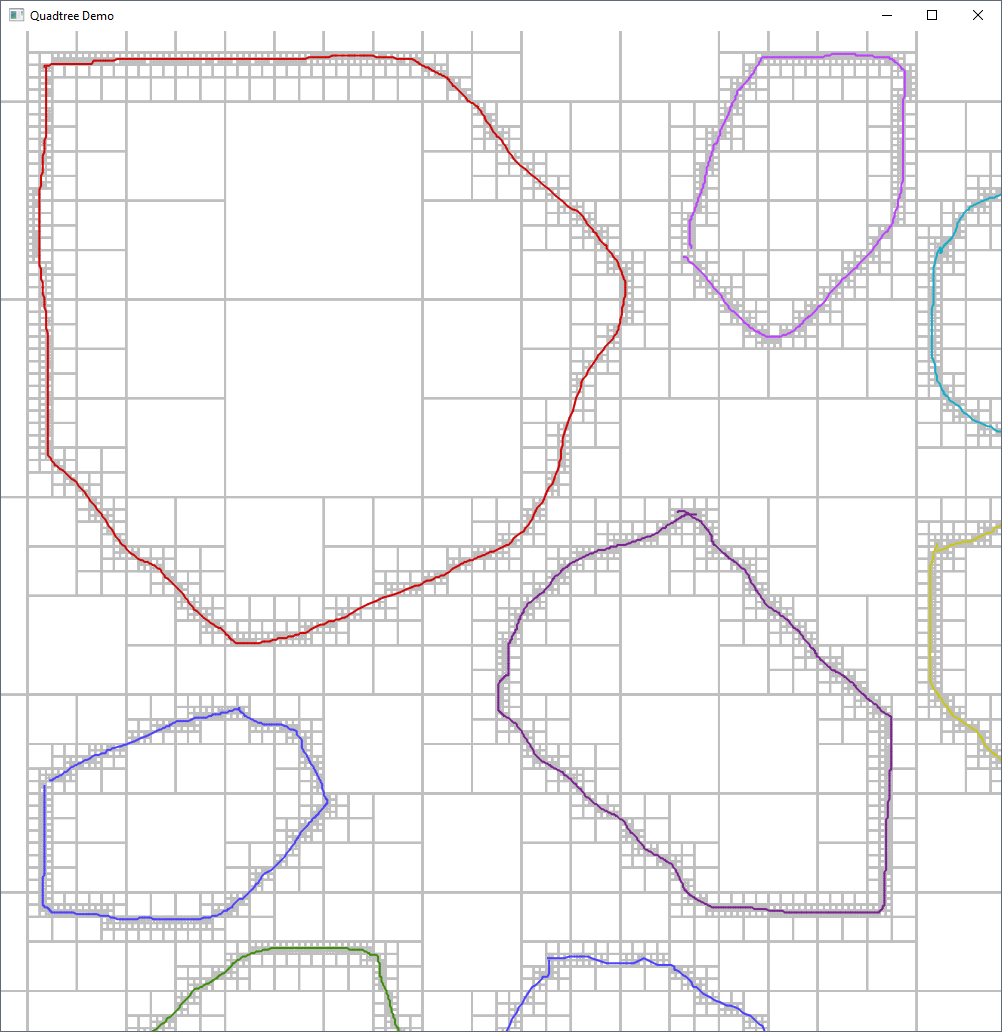
\includegraphics[width=0.35\columnwidth]{pruned-vs-unpruned/4.PNG} }
  \subfloat[][]{
    \label{fig:pruning-2}
    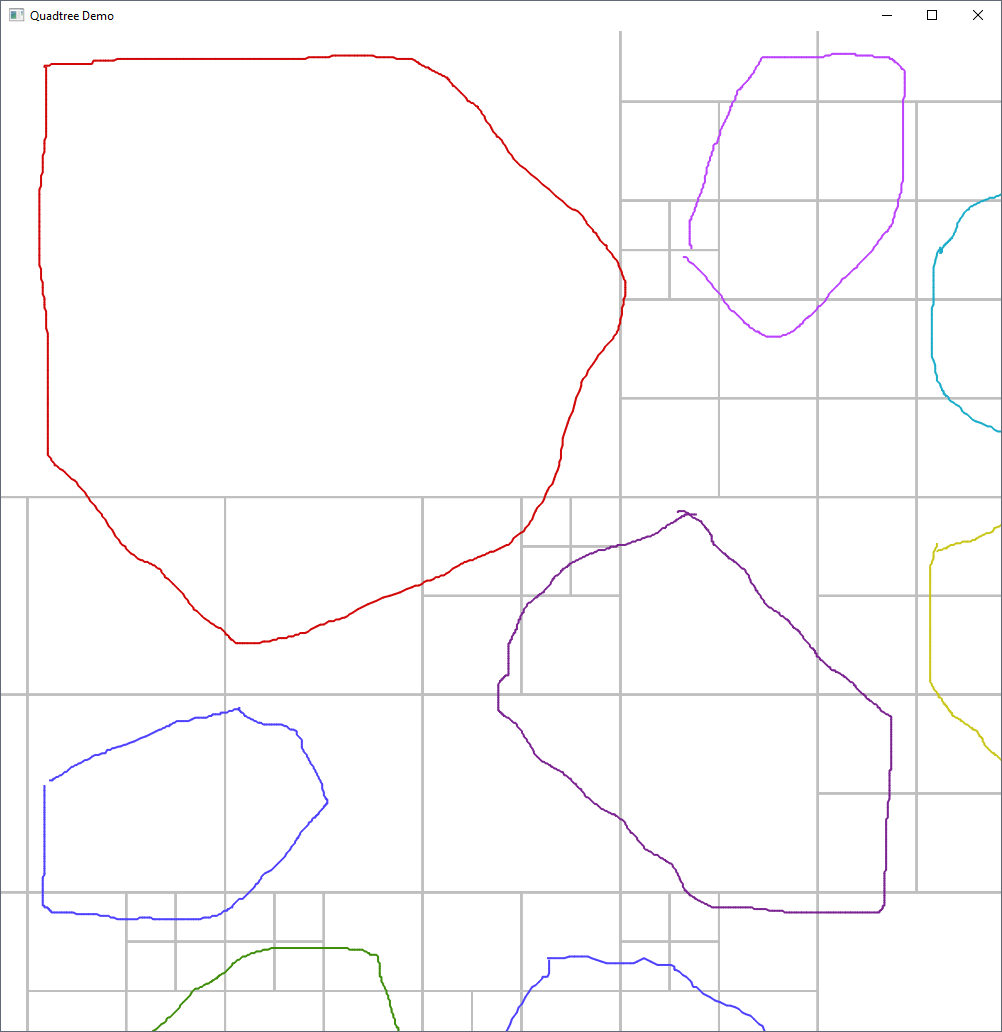
\includegraphics[width=0.35\columnwidth]{pruned-vs-unpruned/5.PNG} }
  \caption{
    \protect\subref{fig:pruning-1} The initial quadtree built on the object vertices, in which no quadtree cell contains more than one vertex, can be far more complex than needed to resolve between objects.
    \protect\subref{fig:pruning-2} After pruning the quadtree. Quadtree cells can contain multiple vertices as long as they all have the same label.
  }
  \label{fig:pruning}
\end{figure}

\subsection{Detect conflict cells}

Let the ``quadtree address'' refer to the unique ID of a quadtree cell $C$ found by concatenating the local addresses of its ancestors from Root to $C$, where the local address is a 2-bit (3-bit in 3D) Morton code. The address of the root cell is defined as the empty string. Figure \ref{fig:conflict-find-4} shows the address of each leaf cell in a quadtree.

We define a bounding cell (BCell) to be the smallest internal quadtree node which entirely contains a given facet. Given a facet defined by $n$ endpoints $P=\{p_1, p_2, \dots, p_n\}$, the quadtree address of the BCell is the longest common prefix of the Morton codes of the points in $P$. If a given LCP is more specific than any quadtree node, i.e., if the LCP lies within a quadtree leaf, we simply take the quadtree address of the leaf that the LCP lies within. This is often the case with pruned quadtrees where entire facets may lie within a quadtree leaf. \red{Please check to make sure I got the changes right.} Figure \ref{fig:data-structures-1} gives the addresses of the BCells of the facets in figure \ref{fig:conflict-find-4}.

We begin by constructing an array \texttt{BCells} and sibling array \texttt{FacetMap} (see figure \ref{fig:data-structures-1}), which is done in parallel over all facets. Each facet $f$ computes the longest common prefix of its vertices and stores the result in \texttt{BCells[$f$]}.

Next we sort the \texttt{BCells} and \texttt{FacetMap} arrays on the \texttt{BCell} values using a parallel radix lexicographical sort (figure \ref{fig:data-structures-2}).% \texttt{BCells} array construction and sorting is done in parallel with the initial Karras quadtree construction.

\begin{figure}
  \centering
  \begin{tikzpicture}
    \node[anchor=south west,inner sep=0,outer sep=0] at (0,0) {
%      \subfloat[][]{
%        \label{fig:conflict-find-1}
%        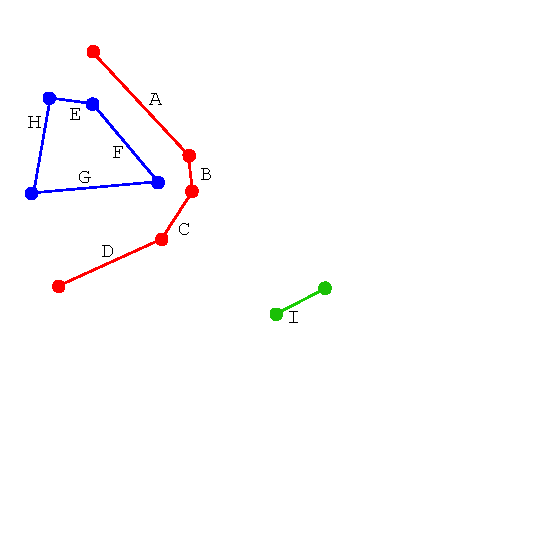
\includegraphics[width=0.44\columnwidth]{conflict-find-1.pdf} } \hfill
      \subfloat[][]{
        \label{fig:conflict-find-2}
        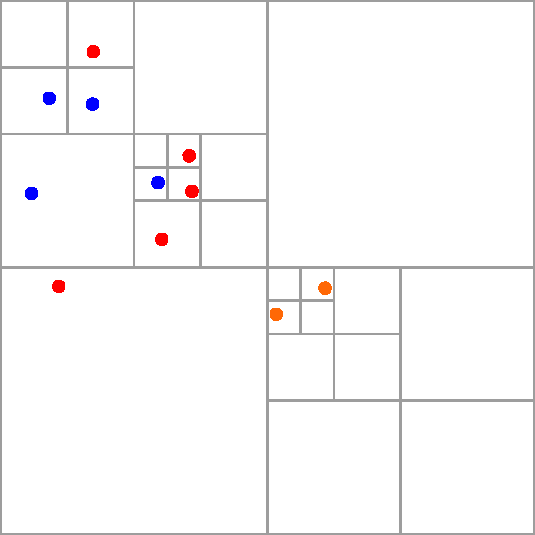
\includegraphics[width=0.44\columnwidth]{conflict-find-2.pdf} } \hfill
      \subfloat[][]{
        \label{fig:conflict-find-4}
        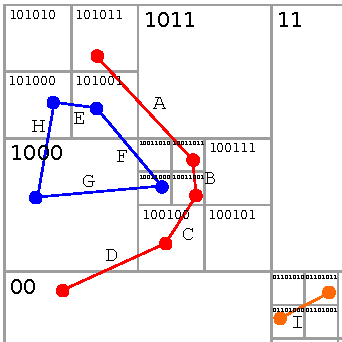
\includegraphics[width=0.44\columnwidth]{conflict-find-4.pdf} } \hfill
%      \subfloat[][]{
%        \label{fig:conflict-find-5}
%        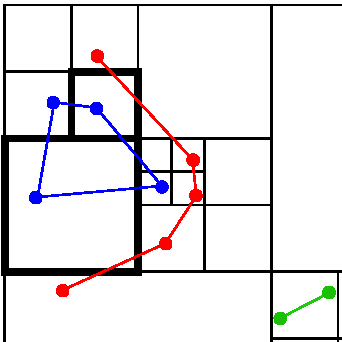
\includegraphics[width=0.44\columnwidth]{conflict-find-5.pdf} }
%      \subfloat[][]{
%        \label{fig:conflict-find-6}
%        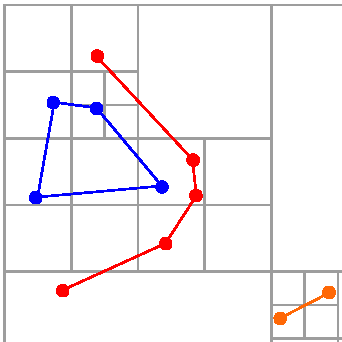
\includegraphics[width=0.44\columnwidth]{conflict-find-6.pdf} }
    };

%    \node[anchor=south west,inner sep=0,outer sep=0] at (0,-4) {
%%      \subfloat[][]{
%%        \label{fig:conflict-find-2}
%%        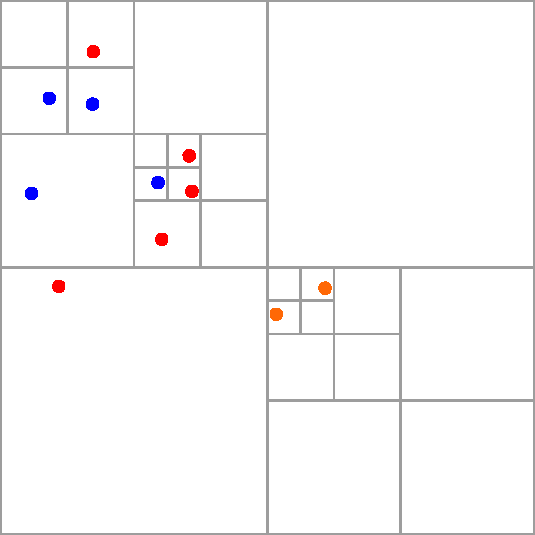
\includegraphics[width=0.44\columnwidth]{conflict-find-2.pdf} } \hfill
%%      \subfloat[][]{
%%        \label{fig:conflict-find-4}
%%        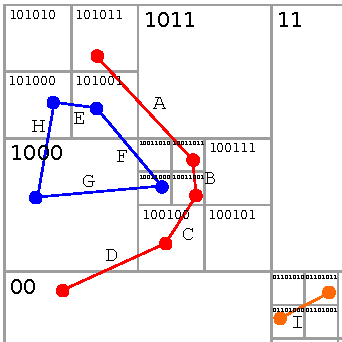
\includegraphics[width=0.44\columnwidth]{conflict-find-4.pdf} } \hfill
%      \subfloat[][]{
%        \label{fig:conflict-find-5}
%        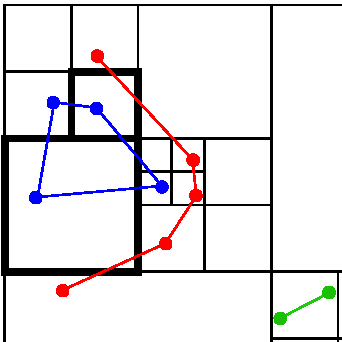
\includegraphics[width=0.44\columnwidth]{conflict-find-5.pdf} }
%      \subfloat[][]{
%        \label{fig:conflict-find-6}
%        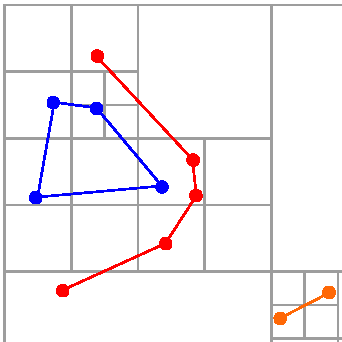
\includegraphics[width=0.44\columnwidth]{conflict-find-6.pdf} }
%    };

    %% single column
    %% small rectangle
    %\draw[red,thick] (4.0,1.7) rectangle (6.55,4.2);
    %% upper-right line
    %\draw[red,thin] (6.55,4.2) -- (11.8,4.2);
    %% lower-left line
    %\draw[red,thin] (4.0,1.7) -- (8.0,0.3);
    %% large rectangle
    %\draw[red,thick] (8.0,0.3) rectangle (11.8,4.2);

%    % spanning column, 0.44 size
%    % small rectangle
%    \draw[red,thick] (1.0,1.7) rectangle (6.55,4.2);
%    % upper-right line
%    \draw[red,thin] (6.55,4.2) -- (11.8,4.2);
%    % lower-left line
%    \draw[red,thin] (4.0,1.7) -- (8.0,0.3);
%    % large rectangle
%    \draw[red,thick] (8.0,0.3) rectangle (11.8,4.2);

%    % two column, .22 size
%    % small rectangle
%    \draw[red,thick] (2.0,1.05) rectangle (3.27,2.25);
%    % upper-right line
%    \draw[red,thin] (3.27,2.25) -- (3.9,2.25);
%    % lower-left line
%    \draw[red,thin] (2.0,1.05) -- (3.9,0.4);
%    % large rectangle
%    \draw[red,thick] (3.9,0.4) rectangle (5.8,2.25);

    % two column, .4 size
    % small rectangle
    \draw[red,thick] (0.0,1.65) rectangle (2.33,4.0);
%    % upper-right line
%    \draw[red,thin] (3.27,2.25) -- (3.9,2.25);
%    % lower-left line
%    \draw[red,thin] (2.0,1.05) -- (3.9,0.4);
%    % large rectangle
%    \draw[red,thick] (3.9,0.4) rectangle (5.8,2.25);
  \end{tikzpicture}



%      \subfloat[][]{
%        \label{fig:conflict-find-2}
%        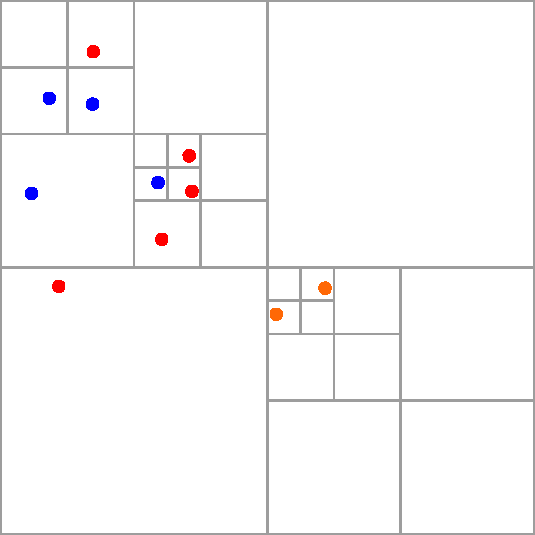
\includegraphics[width=0.44\columnwidth]{conflict-find-2.pdf} } \hfill
%      \subfloat[][]{
%        \label{fig:conflict-find-4}
%        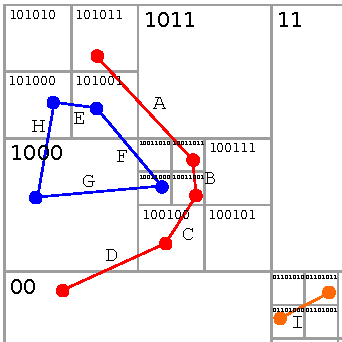
\includegraphics[width=0.44\columnwidth]{conflict-find-4.pdf} } \hfill
      \subfloat[][]{
        \label{fig:conflict-find-5}
        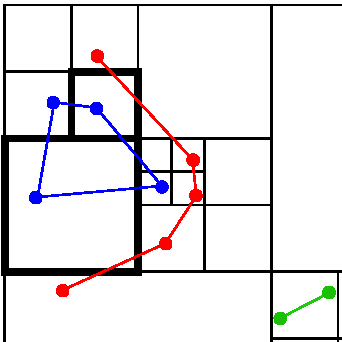
\includegraphics[width=0.44\columnwidth]{conflict-find-5.pdf} }
      \subfloat[][]{
        \label{fig:conflict-find-6}
        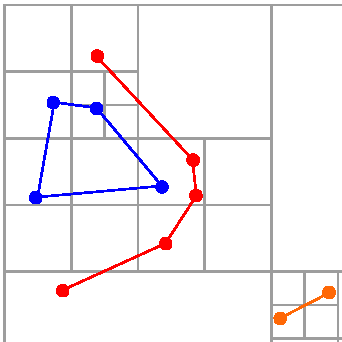
\includegraphics[width=0.44\columnwidth]{conflict-find-6.pdf} }

%      \subfloat[][]{
%        \label{fig:data-structures-1}
%        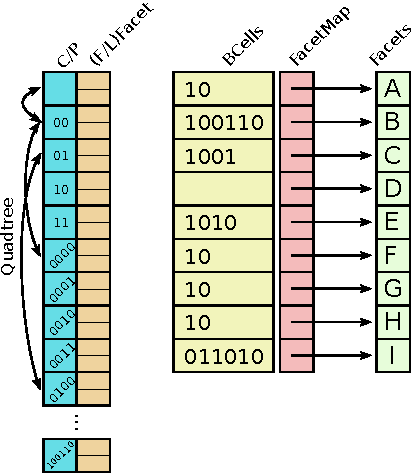
\includegraphics[width=0.38\columnwidth]{data-structures-1.pdf} } \hfill
%      \subfloat[][]{
%        \label{fig:data-structures-2}
%        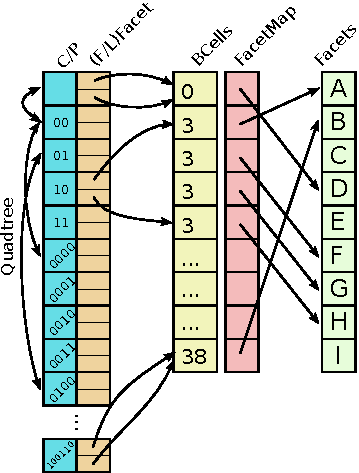
\includegraphics[width=0.38\columnwidth]{data-structures-3.pdf} } \hfill
%      \subfloat[][]{
%        \label{fig:data-structures-3}
%        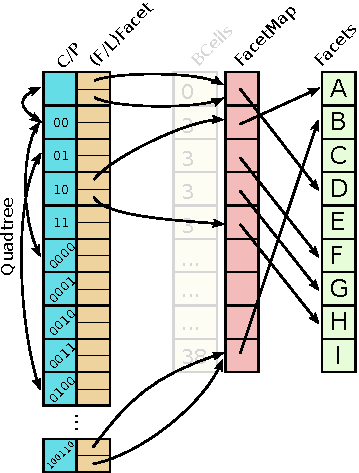
\includegraphics[width=0.38\columnwidth]{data-structures-4.pdf} }
  \caption{
%    \protect\subref{fig:conflict-find-1} We have three objects, blue, red, and green with facets labeled A-I.
    \red{Is the pruning correct?}
    We have three objects, blue, red, and green with facets labeled A-I.
    \protect\subref{fig:conflict-find-2} Initial pruned vertex quadtree.
    \protect\subref{fig:conflict-find-4} Zoomed-in to the region outlined by red in \protect\subref{fig:conflict-find-2} and showing the boundary cell (BCell) computation for each facet. %These pairs are given in figure \protect\subref{fig:data-structures-1}.
    \protect\subref{fig:conflict-find-5} Conflict cells, which intersect more than one object, are highlighted.
    \protect\subref{fig:conflict-find-6} The new quadtree after conflict resolution.
%    \protect\subref{fig:data-structures-1} The bounding cells (BCells) are stored in an array initially sorted on facet index (letters are used here for clarity). The quadtree array elements are structures which store child and parent pointers (``C/P'' in the figure).
%    \protect\subref{fig:data-structures-2} We sort the BCells array using a parallel radix sort on BCell address for fast indexed access. We then, in parallel on each element of the BCells array, store the BCells/FacetMap indices of the first and last facets in a given quadtree cell in \texttt{FFacet} and \texttt{LFacet}, respectively.
%\protect\subref{fig:data-structures-3} For a given quadtree cell, we can find all contained facets for use in algorithm \ref{alg:find-conflict-cells}.
  }
  \label{fig:conflict-find}
\end{figure}

\begin{figure}
  \centering
      \subfloat[][]{
        \label{fig:data-structures-1}
        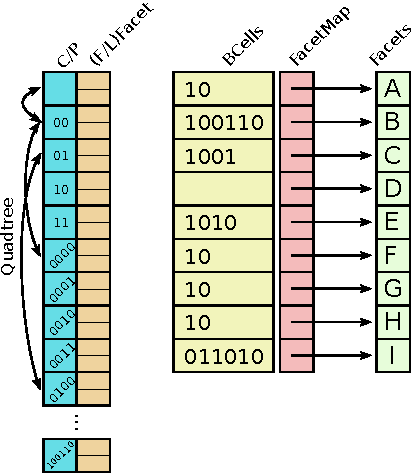
\includegraphics[width=0.32\columnwidth]{data-structures-1.pdf} }
      \subfloat[][]{
        \label{fig:data-structures-2}
        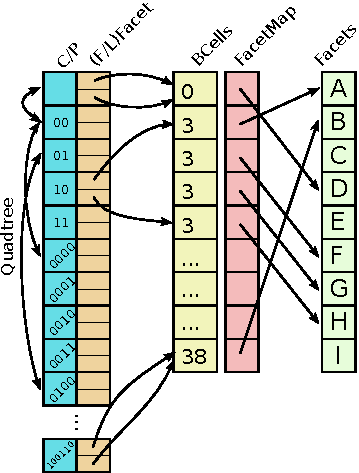
\includegraphics[width=0.32\columnwidth]{data-structures-3.pdf} }
      \subfloat[][]{
        \label{fig:data-structures-3}
        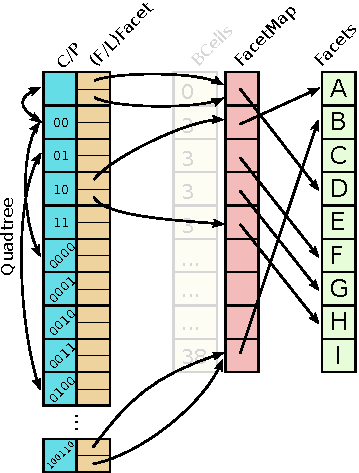
\includegraphics[width=0.32\columnwidth]{data-structures-4.pdf} }
  \caption{
    \protect\subref{fig:data-structures-1} The bounding cells (BCells) are stored in an array initially sorted on facet index (letters are used here for clarity). The quadtree array elements are structures which store child and parent pointers (``C/P'' in the figure).
    \protect\subref{fig:data-structures-2} We sort the BCells array using a parallel radix sort on BCell address for fast indexed access. We then, in parallel on each element of the BCells array, store the BCells/FacetMap indices of the first and last facets in a given quadtree cell in \texttt{FFacet} and \texttt{LFacet}, respectively.
\protect\subref{fig:data-structures-3} For a given quadtree cell, we can find all contained facets for use in algorithm \ref{alg:find-conflict-cells}.
  }
  \label{fig:data-structures}
\end{figure}

Then we use the \texttt{BCells} array and quadtree data structure to find the conflict cells using algorithm \ref{alg:find-conflict-cells}. We process each leaf cell $L$ in parallel (line \ref{alg:L}). First, we set $L$'s color to $-1$ (uninitialized). We then investigate each ancestor $A$ of $L$ (line \ref{alg:A}) by using the \texttt{Parent} field in the quadtree data structure. Using the \texttt{FFacet} and \texttt{LFacet} fields, we find, respectively, the first and (inclusive) last of possibly multiple facets bounded by $A$ (line \ref{alg:i}). The \texttt{FacetMap} array is used to find all facets bounded by bounding cell $A$ (line \ref{alg:f}). Any facet $f$ for which $A$ is the bounding cell could potentially intersect the leaf cell $L$. We test for intersection between $f$ and $L$ and store the first two facets of differing color (lines \ref{alg:7}-\ref{alg:16}). If at the conclusion of execution $L$.color is equal to $-2$ then $L$ is a conflict cell and must be resolved.

\algorithmspace
\begin{algorithm}
  \DontPrintSemicolon
  \LinesNumbered
  \KwIn{Quadtree}
  \BlankLine
  \ForPar{leaf cell $L$}{ \label{alg:L}
    $L$.color = -1\;
    \ForEach{cell $A$ in \directAncestors{$L$}}{  \label{alg:A}
      \ForEach{i in \{FFacet[A]$\dots$LFacet[A]\}}{ \label{alg:i}
%      i := Quadtree[$A$].Facets\; \label{alg:i}
%      \While{BCells[i].Cell\_ID = Address($A$)}{
%        $f$ := Facets[BCells[i].Facet\_idx]\; \label{alg:f}
        $f$ := Facets[FacetMap[i]]\; \label{alg:f}
        \If{$f$ intersects $L$}{ \label{alg:7}
          \If{$L$.color == -1} {
            $L$.color = $f$.color\;
            $L$.facet[0] = $f$\;
          }
          \ElseIf{$L$.color $\ne$ $f$.color} {
            $L$.color = -2\;
            $L$.facet[1] = $f$\;
          }
        } \label{alg:16}
      }
    }
  }
\caption{FIND\_CONFLICT\_CELLS}
\label{alg:find-conflict-cells}
\end{algorithm}
\algorithmspace

\subsection{Resolve conflict cells}
\label{sec:resolve}

\begin{figure}
  \centering
  \subfloat[][]{
    \label{fig:conflict-resolution-x}
    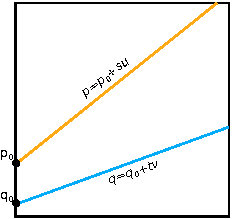
\includegraphics[width=0.35\columnwidth]{conflict-resolution-x.pdf} }
  \subfloat[][]{
    \label{fig:conflict-resolution-even}
    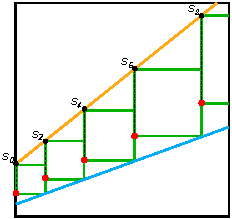
\includegraphics[width=0.35\columnwidth]{conflict-resolution-even.pdf} }\\
  \subfloat[][]{
    \label{fig:conflict-resolution-all}
    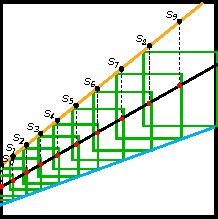
\includegraphics[width=0.35\columnwidth]{conflict-resolution-all.pdf} }
  \subfloat[][]{
    \label{fig:conflict-resolution-quadtree}
    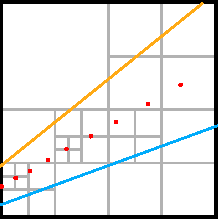
\includegraphics[width=0.35\columnwidth]{conflict-resolution-octree.pdf} }\\
  \subfloat[][]{
    \label{fig:conflict-resolution-adjacent-even}
    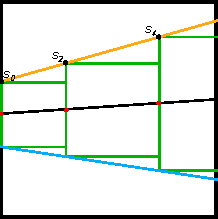
\includegraphics[width=0.35\columnwidth]{conflict-resolution-adjacent-even.pdf} }
  \subfloat[][]{
    \label{fig:conflict-resolution-adjacent-all}
    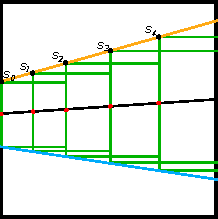
\includegraphics[width=0.35\columnwidth]{conflict-resolution-adjacent-all.pdf} }
  \caption{
    \protect\subref{fig:conflict-resolution-x} A conflict cell with two lines from different objects.
    \protect\subref{fig:conflict-resolution-even} Fitting boxes such that any box intersecting both lines contains at least one sample (red dots).
    \protect\subref{fig:conflict-resolution-even} Fitting boxes such that any box intersecting both lines contains at least two samples. This ensures that a quadtree built from the samples using Karras' algorithm (panel \protect\subref{fig:conflict-resolution-quadtree}) will have no leaf cells that intersect both lines, ensuring that the new quadtree is locally free of conflict cells.
  }
  \label{fig:conflict-resolution}
\end{figure}

We present a conflict cell resolution algorithm for pairs of lines in 2D. For a conflict cell $C$, our approach is to find sample points inside the cell such that no leaf cells in a quadtree constructed over the sample points intersect both lines. In this section we derive equation \eqref{eqn:num-samples} which computes the number of samples required to resolve the cell. We also derive equation \eqref{eqn:sample} which computes the samples themselves. The power of our approach lies in the fact that both expressions are closed-form and neither one is iterative, so we can evaluate the first in parallel over leaf cells and the second in parallel over all samples that we need to compute.

To resolve a conflict cell $C$, we consider pairs of lines of differing labels that intersect $C$. Figure \ref{fig:conflict-resolution-x} shows two lines

\begin{align}
q(t) &= q = q_0 + tv \label{eqn:q} \\
r(f) &= r = r_0 + fw \label{eqn:r}
\end{align}
along with a line
\begin{align}
p(s) &= p = p_0 + su \label{eqn:p}
\end{align}
that bisects $q$ and $r$. Our strategy will be to sample points $P$ on $p(s)$ (figure \ref{fig:conflict-resolution-quadtree}) such that a quadtree built on $S \cup P$ will completely ``separate'' $q$ and $r$, i.e., no descendent leaf of $C$ will intersect both $q$ and $r$. We do this by ensuring that $P$ is sampled such that every box that intersects both $q$ and $r$ also intersects at least two points in $P$. Because Karras' algorithm guarantees that every leaf cell intersects at most one point, we know that no leaf cell will intersect $q$ and $r$ and thus no leaf cell will be a conflict cell. We will find a series of boxes such that each box's left-most intersection with $p(s)$ is a sample point meeting the above criterion. In the following discussion, $p^x$ and $p^y$ refer to the $x$ and $y$ coordinates of point $p$, respectively.

We consider only cases where the slope of $p$ is in the range $0 \le m \le 1$. All other instances can be transformed to this case using rotation and reflection. We begin by fitting the smallest box centered on a point $p$ that intersects both $q$ and $r$. We break the problem into two cases:
%\begin{tightenumerate}
\begin{enumerate}
 \item The \textit{opposite} case (see figure \ref{fig:conflict-resolution-even}) is where $w^y > 0$, so each box intersects $q$ and $r$ at its top-left and bottom-right corners, respectively.
 \item In the \textit{adjacent} case (see figure \ref{fig:conflict-resolution-adjacent-even}), $w^y < 0$, so the line intersections are adjacent at the top-left and bottom-left corners of the box.
%\end{tightenumerate}
\end{enumerate}

\subsubsection{Finding $a(s)$ -- \textit{opposite} case}

Given a point $p(s)$, we wish to find $a=a(s)$, which will give us the starting $x$ coordinate for the next box. Consider the top-left corner of the box $q(t(s))=q(t)$ and the bottom-right corner $r(f(s))=r(f)$.

Because $p^x(s)=q^x(t)$,
\begin{equation}
t = \frac{p^x(s)-q_0^x}{v^x} = \frac{p_x^x-q_0^x+su^x}{v^x} \label{eqn:t}
\end{equation}
Because our boxes are square,
\begin{equation}
r(f) = r_0+fw = q_0+tv+a\begin{bmatrix}1\\-1\end{bmatrix} \label{eqn:ro}
\end{equation}
From \eqref{eqn:ro},
\begin{align}
f &= \frac{1}{w^y}(q_0^y+tv^y-a-r_0^y) \label{eqn:f} \\
a &= r_0^x+fw^x-q_0^x-tv^x \label{eqn:a1o}
\end{align}
Substituting equations \eqref{eqn:t} and \eqref{eqn:f} into equation \eqref{eqn:a1o} and solving for $a$,
\begin{equation}
a(s) = \hat{\alpha}_o s + \hat{\beta}_o \label{eqn:ao}
\end{equation}
where
\begin{equation}
\hat{\alpha}_o = \frac{u^x|w \times v|}{v^x(w^x+w^y)}
\end{equation}
and
\begin{equation}
\hat{\beta}_o = \frac{|w \times v|(p_0^x-q_0^x) + v^x(|r_0 \times w| + |w \times q_0|)}{v^x(w^x+w^y)}
\end{equation}

\subsubsection{Finding $a(s)$ -- \textit{adjacent} case}

Consider the top-left corner of the box $q(t(s))=q(t)$ and the bottom-left corner $r(f(s))=r(f)$. $r(f)$ is now defined as
\begin{equation}
r(f) = r_0+fw = q_0+tv+a\begin{bmatrix}0\\-1\end{bmatrix} \label{eqn:ra}
\end{equation}
Equations \eqref{eqn:t} and \eqref{eqn:f} remain the same while \eqref{eqn:a1o} becomes
\begin{equation}
0 = r_0^x+fw^x-q_0^x-tv^x \label{eqn:a1a}
\end{equation}
Substituting equations \eqref{eqn:t} and \eqref{eqn:f} into equation \eqref{eqn:a1a} and solving for $a$,
\begin{equation}
a(s) = \hat{\alpha}_a s + \hat{\beta}_a \label{eqn:aa}
\end{equation}
where
\begin{equation}
\hat{\alpha}_a = \frac{u^x}{v^xw^x}
\end{equation}
and
\begin{equation}
\hat{\beta}_a = \frac{w^x(p_0^x-q_0^x)+|w \times q_0| + |r_0 \times w|}{w^x}
\end{equation}


%
%
%Because $p^x(s)=q^x(t)$,
%\begin{equation}
%t = \frac{p^x(s)-q_0^x}{v^x} = \frac{p_x^x-q_0^x+su^x}{v^x} \label{eqn:t}
%\end{equation}
%Because our boxes are square,
%\begin{equation}
%r(f) = r_0+fw = q_0+tv+a
%\begin{bmatrix}
%1\\-1
%\end{bmatrix}
%\label{eqn:r}
%\end{equation}
%From \eqref{eqn:r},
%\begin{align}
%f &= \frac{1}{w^y}(q_0^y+tv^y-a-r_0^y) \label{eqn:f} \\
%a &= r_0^x+fw^x-q_0^x-tv^x \label{eqn:a1}
%\end{align}
%Substituting equations \eqref{eqn:t} and \eqref{eqn:f} into equation \eqref{eqn:a1} and solving for $a$,
%\begin{equation}
%a = \alpha s + \beta
%\end{equation}
%where
%\begin{equation}
%\alpha = \frac{u^x|w \times v|}{v^x(w^x+w^y)}
%\end{equation}
%and
%\begin{equation}
%\beta = \frac{|w \times v|(p_0^x-q_0^x) + v^x(|r_0 \times w| + |w \times q_0|)}{v^x(w^x+w^y)}
%\end{equation}
%
%Consider a box with edge length $a_0$ centered on a point $p_0 \in p$. We first find $p$, which is the line that is equidistant from $q$ and $r$ along the diagonal vector $\gamma = (1, -1)$. Given some point $q(t)$,
%\begin{equation}
%q_0+tv + \lambda\gamma = r_0+fw \\
%\end{equation}
%Solving for $\lambda$,
%\begin{align}
%f &= \frac{1}{w^y}(q_0^y+tv^x-\lambda-r_0^y) \\
%\lambda &= r_0^x + fw^x-q_0^x-tv^x \\
%        &= r_0^x+\frac{w^x}{w^y}(q_0^y+tv^y-\lambda-r_0^y) - q_0^x-tv^x \\
%        &= \frac{1}{w^x+w^y}(r_0^xw^y+q_0^yw^x-r_0^yw^x-q_0^xw^y+t(v^yw^x-v^xw^y)
%\end{align}
%The vector $u = p - p_0$. We obtain $p$ from $q(0)$, by finding $\lambda/2$.
%\begin{align}
%p = q(0) + \frac{\lambda}{2}\gamma
%\end{align}
%We get $p_0$ by finding the intersection between the two lines. If they are parallel then we find two points $p$ using $q(0)$ and $q(1)$.
%
%To find $a$,
%\begin{align} 
%p^x-\frac{a}{2} &= q^x \\
%p^y+\frac{a}{2} &= q^y
%\end{align}
%Substituting equation \eqref{eqn:q},
%\begin{align} 
%t = \frac{p^x-a/2-q_0^x}{v^x} \\
%t = \frac{p^y+a/2-q_0^y}{v^y}
%\end{align}
%which leads to
%\begin{align} 
%\frac{p^x-a/2-q_0^x}{v^x} &= \frac{p^y+a/2-q_0^y}{v^y}
%\end{align}
%Solving for $a$,
%\begin{align}
%\label{eqn:plain_a}
%a &= \frac{2(p^xv^y-q_0^xv^y-p^yv^x+q_0^yv^x)}{v^x+v^y}
%\end{align}
%$a$ is a parametric function in $s$, so using equations \eqref{eqn:plain_a} and \eqref{eqn:p},
%\begin{align}
%a(s) &= \frac{2((p_0^x+su^x)v^y-q_0^xv^y-(p_0^y+su^y)v^x+q_0^yv^x)}{v^x+v^y} \\
%     &= s\frac{2(u^xv^y-u^yv^x)}{v^x+v^y} + \frac{2(p_0^xv^y-q_0^xv^y-p_0^yv^x+q_0^yv^x)}{v^x+v^y} \label{eqn:a}
%\end{align}
%Figure \ref{fig:conflict-resolution-even} shows that we will find a series of points $P=p(s_i)$ such that
%\begin{equation}
%p^x(s_i) = p^x(s_{i-2})+a(s_{i-2}) \label{eqn:p_s}
%\end{equation}
%Using equations \eqref{eqn:p}, \eqref{eqn:a} and \eqref{eqn:p_s},
%\begin{align}
%p_0^x+s_iu^x = p_0^x+s_{i-2}u^x+s_{i-2}\frac{2(u^xv^y-u^yv^x)}{v^x+v^y} + \frac{2(p_0^xv^y-q_0^xv^y-p_0^yv^x+q_0^yv^x)}{v^x+v^y}
%\end{align}
%Solving for $s_i$,
%\begin{equation}
%\label{eqn:si_rec}
%s_i = s_{i-2}\alpha + \beta
%\end{equation}
%where
%\begin{align}
%%\alpha &= \frac{u^xv^x+3u^xv^y-2u^yv^x}{u^x(v^x+v^y)}
%\alpha &= 1+\frac{2(u^xv^y-u^yv^x)}{u^x(v^x+v^y)} \\
%\beta &= \frac{2(p_0^xv^y-q_0^xv^y-p_0^yv^x+q_0^yv^x)}{u^x(v^x+v^y)}
%\end{align}

\subsubsection{Sampling}
In both the \textit{opposite} and the \textit{adjacent} cases, $a(s)$ is of the form $a(s) = \hat{\alpha} s + \hat{\beta}$. We now use $a(s)$ to construct a sequence of values $S = \{s_0, s_1, s_2, \dots, s_n\}$ that meet our sampling criterion. We first construct the even samples (see figures \ref{fig:conflict-resolution-even} and \ref{fig:conflict-resolution-adjacent-even}). Given a starting point $p(s_0)$,
\begin{equation}
p^x(s_{i+2}) = p^x(s_i) + a(s_i)
\end{equation}
Substituting in equations \eqref{eqn:p} and \eqref{eqn:ao}/\eqref{eqn:aa},
\begin{equation}
p_0^x + s_{i+2}u^x = p_0^x + s_i + \hat{\alpha} s_i + \hat{\beta}
\end{equation}
Solving for $s_{i+2}$ gives the recurrence relation
\begin{equation}
s_{i+2} = \alpha s_i + \beta \label{eqn:recurrence}
\end{equation}
where
\begin{equation}
\alpha = 1 + \frac{\hat{\alpha}}{u^x}
\end{equation}
and
\begin{equation}
\beta = \frac{\hat{\beta}}{u^x}
\end{equation}

Constructing the odd samples is identical, except that we start at
\begin{equation}
s_1 = \left(1+\frac{\hat{\alpha}}{2u^x}\right)s_0 + \frac{\hat{\beta}}{2}
\end{equation}
which is the point in the center of the first box in the x-dimension.

We solve the recurrence relation \eqref{eqn:recurrence} using the characteristic polynomial to yield
\begin{equation}
s_i = k_1 + k_2 \alpha^i \label{eqn:sample}
\end{equation}
where the $k$ variables are split into those for even values of $i$ and those for odd values of $i$, and are given as
\begin{align}
k_1^{even} &= \frac{\beta}{1-\alpha} \\
k_1^{odd} &= \frac{\beta}{1-\alpha} \\
k_2^{even} &= \frac{\alpha s_0 + \beta - s_0}{\alpha-1} \\
k_2^{odd} &= \frac{\alpha s_1 + \beta - s_1}{\alpha-1}
\end{align}
The last step to formulating $P$ for parallel computation is to determine how many samples we will need. Let $p(s_{exit})$ be the point at which the line $p$ exits the cell.
\begin{align}
k_1+k_2\alpha^i < s_{exit}
\end{align}
results in
\begin{align}
i < \log_{\alpha}\frac{s_{exit}-k_1}{k_2} \label{eqn:num-samples}
\end{align}

\subsubsection{Iteration}
\label{sec:iterate}

Because conflict cell resolution only considers two facets at a time, we may have to iterate multiple times if more than two facets intersect a given cell. If new sample points were found then we add them to the current set $S$ of sample points and return to building the quadtree from points (section \ref{sec:build-initial-quadtree}). We finish when the only conflicts identified are at the maximum depth.

\subsection{Optimality}
\red{Check this}
Define an optimal quadtree to be one in which only conflict nodes have children, and let an optimal quadtree's size be $n$ total nodes. Our iterative sampling algorithm results in a quadtree that has a size within a constant factor of $n$ in the worst case (see figure \ref{fig:optimality}). We omit the proof as well as an average case analysis because optimality can be achieved by simply performing one final pruning step (see section \ref{sec:pruning}).

\begin{figure}
  \centering
  \subfloat[][]{
    \label{fig:optimality-good}
    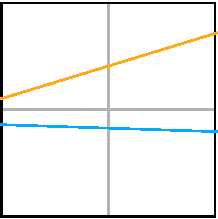
\includegraphics[width=0.25\columnwidth]{optimality-good.pdf} }
  \subfloat[][]{
    \label{fig:optimality-bad}
    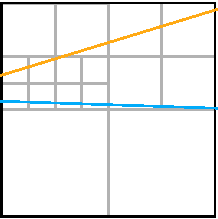
\includegraphics[width=0.25\columnwidth]{optimality-bad.pdf} }
  \subfloat[][]{
    \label{fig:optimality-bad-all}
    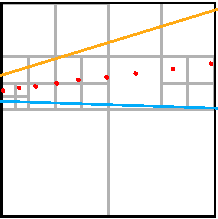
\includegraphics[width=0.25\columnwidth]{optimality-bad-all.pdf} }
  \caption{
    Best and worst cases given two lines. The same number of conflict resolution samples are generated regardless of where the lines are located.
    \protect\subref{fig:optimality-good} Base case: two lines can be resolved by a single quadtree subdivision.
    \protect\subref{fig:optimality-bad} Worst case: the same two lines translated slightly in $y$ now require five subdivisions to be resolved.
    \protect\subref{fig:optimality-bad-all} The number of cells generated from the shown resolution samples is within a constant factor of the worst case.
  }
  \label{fig:optimality}
\end{figure}

\subsection{Complexity analysis}

Let $M = |F|$ and $N = |V|$, where $F$ are the object facets and $V$ are the object vertices. Let $D$ be the depth of the quadtree. In this analysis we assume sufficient parallel units to maximize parallelization.

%\vspace{2mm}
%\paragraph{Time complexity}
\subsubsection{Time complexity}

%\begin{tightenumerate}
\begin{enumerate}
\item Build quadtree using Karras' algorithm \cite{karras2012maximizing}, including pruning - $O(D)$. \red{How about this?}
\item Detect conflict cells
%  \begin{tightenumerate}
  \begin{enumerate}
  \item Build BCells array - $O(D)$. Building of the array runs in parallel for each facet $f$. The facet looks at each vertex (we assume simplices with a constant number of dimensions), computes Morton codes and finds the longest common prefix among vertices. This requires looking at each bit, of which there are $O(D)$.
  \item Sort BCells array - \red{Shouldn't the Big O here be $O(D)$?} $O(\log{M})$. The array has $M$ elements, and we use a parallel radix sort with $\log$ complexity.
  \item Index BCells with quadtree data structure - $O(D)$. This runs in parallel on leaf cell IDs and each kernel requires a search of the quadtree for a given cell ID, taking at most $D$ steps.
  \item Find facets that intersect each leaf cell - Worst case $O(M+D)$, average case $O(D)$. In unusual datasets, a single leaf cell will be intersected by $O(M)$ facets. On average, however, leaf cells intersect a small number of facets, and thus this step is dominated by the depth $D$ of the quadtree due to visiting each ancestor of the leaf cell.
%  \end{tightenumerate}
  \end{enumerate}
\item Resolve conflict cells
%  \begin{tightenumerate}
  \begin{enumerate}
  \item Compute new sample points - $O(1)$. The first step computes, in parallel over conflict cells, the number of samples required to resolve the cell using equation \eqref{eqn:num-samples}. The second step is to compute the samples themselves, which is done in parallel over all new samples to be computed, using equation \eqref{eqn:sample}.
  \item $S \leftarrow S \cup S'$ - $O(1)$.
%  \end{tightenumerate}
  \end{enumerate}
\item Iterate - $O(Q)$ iterations. In the worst case, all facets intersect a single cell, requiring potentially $Q=O(M^2)$ iterations. In our testing, $Q$ has not exceeded 4.
%\end{tightenumerate}
\end{enumerate}

The final complexity of each iteration is $O(M+D)$ worst case and $O(\log{M}+D)$ average case. In practice we must fix the depth of the quadtree to a constant value in order to use a predetermined integer size for the Morton codes, which brings the average case complexity to $O(\log{M})$. Taking iteration into account, the final complexity is $(Q\log{M})$ average case.

%\vspace{2mm}
%\paragraph{Space complexity}
\subsubsection{Space complexity}

The primary data structures are shown in figure \ref{fig:data-structures-1}. The quadtree data structure is size $O(|S|)$ and the remaining arrays are of size $M$. As $|S| \ge M$, our final space complexity is $O(|S|)$. The number of samples in $S$ depends on the dataset. In 2D, in the worst case, the facets can form an arrangement of maximum number of intersections, which is $M(M-1)/2 = O(M^2)$. If this is the case then we subdivide to the maximum quadtree depth at each intersection, causing a quadtree of size $O(DM^2)$. %In our testing, our quadtrees have never exceeded a size of \red{fill this in with experimental results}.

%-------------------------------------------------------------------------------
% Results
%-------------------------------------------------------------------------------
\section{Results and conclusions}
Our implementation\footnote{
Source code will be made available at our website. %is available at \url{http://cedmav.org/research/project/33-gvds.html}.
}
of the algorithm supports polygons and polylines which needn't be manifold or connected. All tests were run on a Razer Blade Stealth with an Intel i7 6500u 3.10 GHz dual core processor, 8 GB of memory and an Nvidia GTX 1070 graphics card. Figure \ref{fig:results-toy} shows results a simple toy dataset showing conflict cell detection and resolution. A very complex dataset with many objects at very different scales is shown in figure \ref{fig:results-maze}. It demonstrates that our method can handle datasets far beyond the memory limits of uniform grid approaches while still fully resolving between objects. The gears dataset (figure \ref{fig:gears}) again shows a large domain-to-object-spacing ratio, as well as non-convexities. The vascular dataset shown in figure \ref{fig:vascular} demonstrates our method on polylines derived from biological image data, which is often noisy with non-manifoldness and intersections. Table \ref{tab:timings} shows timings for our implementation compared to the previous state-of-the-art. Our implementation is significantly faster and also generates fewer quadtree cells.

\begin{figure}
  \centering
  \subfloat[][]{
    \label{fig:simple-conflicts}
    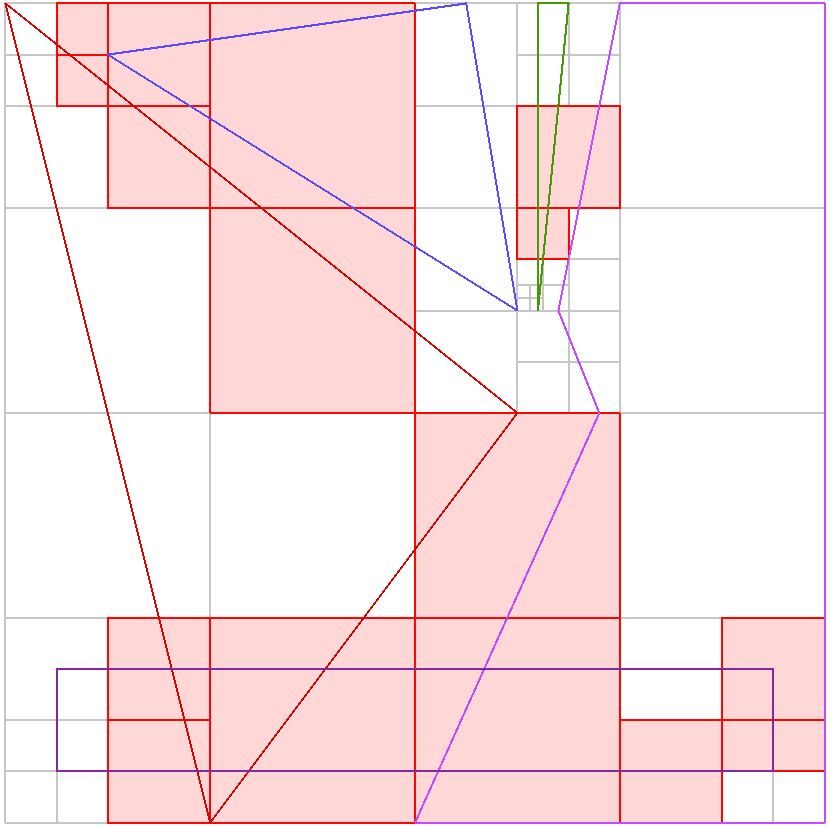
\includegraphics[width=0.31\columnwidth]{simple-conflict.png} }
  \subfloat[][]{
    \label{fig:simple-samples}
    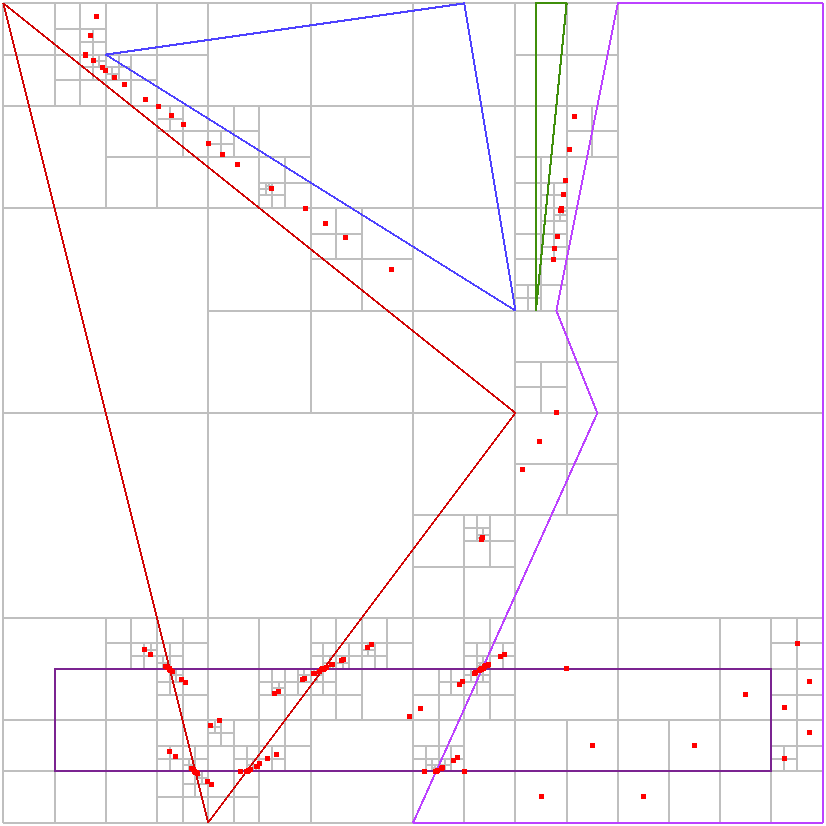
\includegraphics[width=0.31\columnwidth]{simple-samples.png} }

  \caption{
    \protect\subref{fig:simple-conflicts} A toy dataset showing conflict cells after building the quadtree from object vertices.
    \protect\subref{fig:simple-samples} The toy dataset showing how samples are collected.
  }
  \label{fig:results-toy}
\end{figure}

\begin{figure}
  \centering
  \subfloat[][]{
    \label{fig:ut1-samples}
    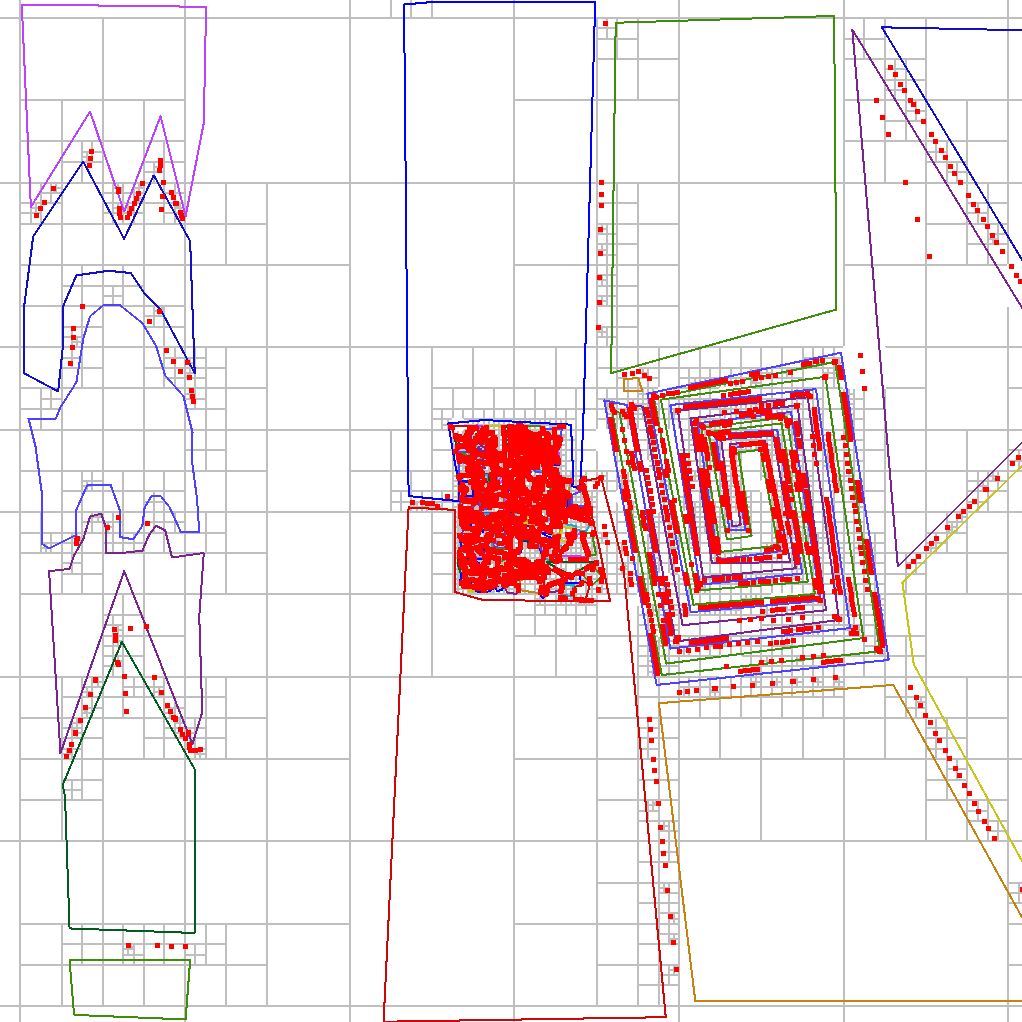
\includegraphics[width=0.31\columnwidth]{ut1-samples.png} }
  \subfloat[][1x zoom]{
    \label{fig:ut1}
    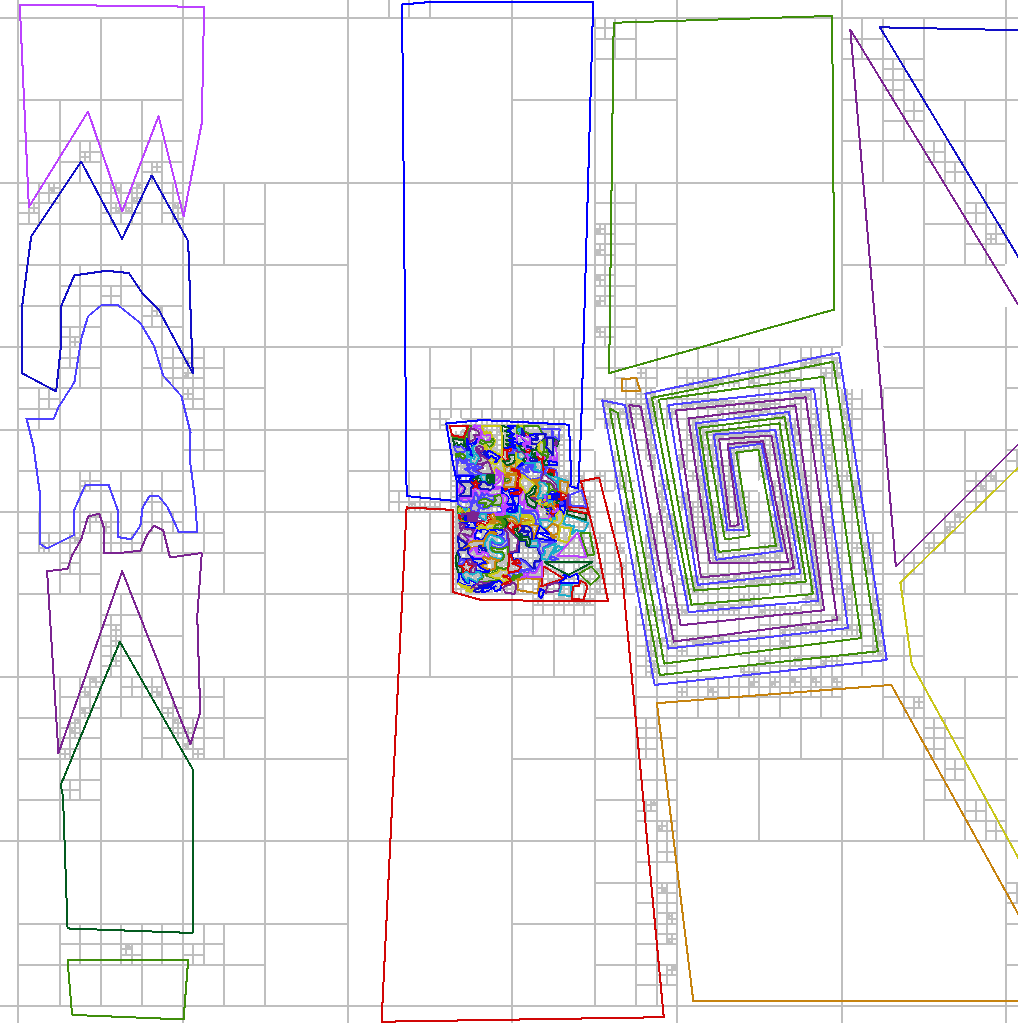
\includegraphics[width=0.31\columnwidth]{ut1.png} }
  \subfloat[][16x zoom]{
    \label{fig:ut2}
    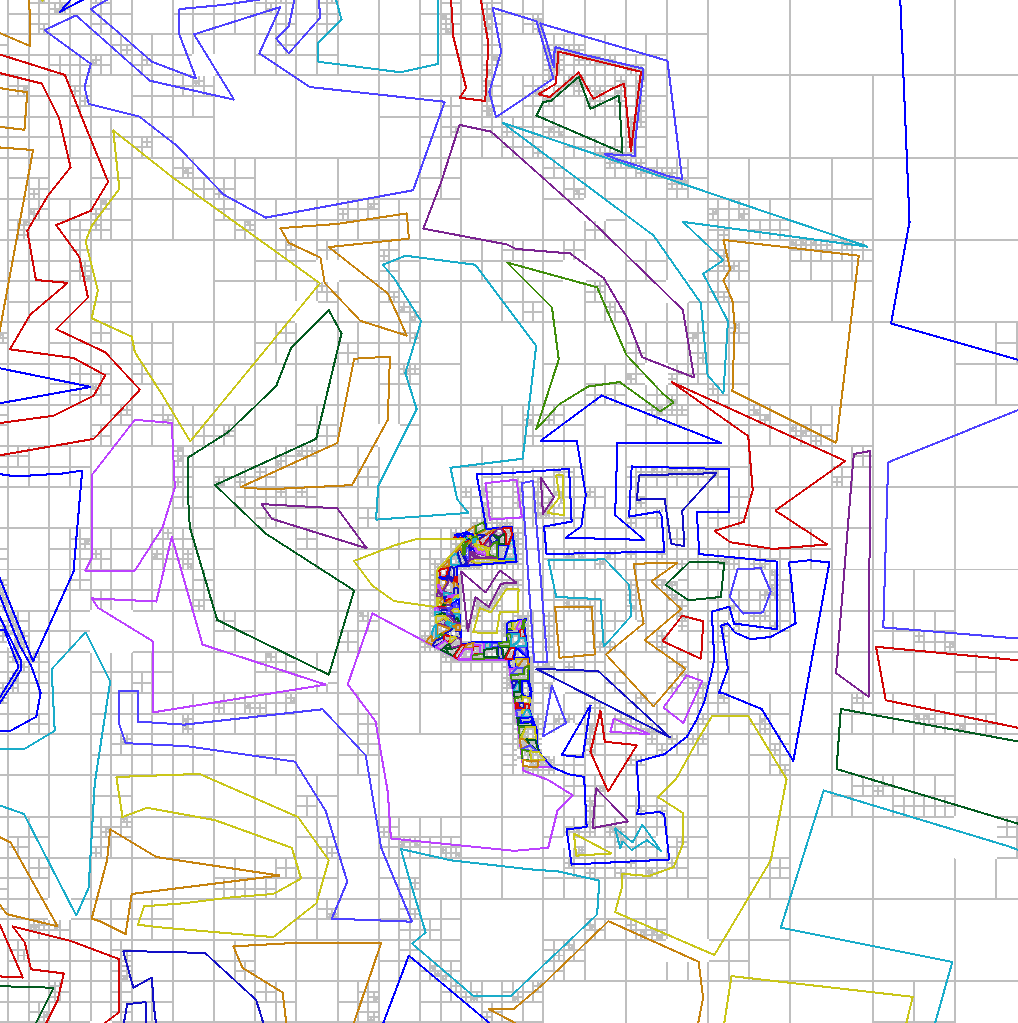
\includegraphics[width=0.31\columnwidth]{ut2.png} } \\
  \subfloat[][256x zoom]{
    \label{fig:ut3}
    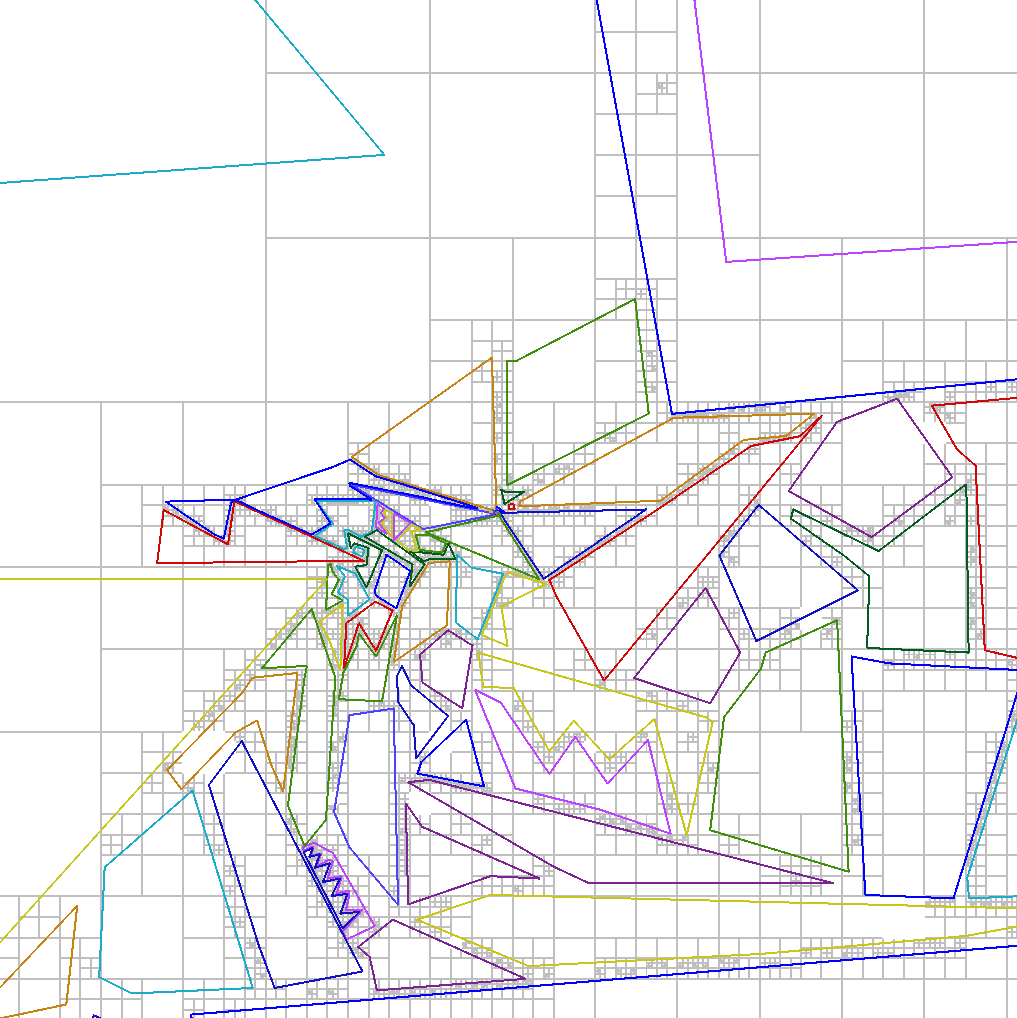
\includegraphics[width=0.31\columnwidth]{ut3.png} }
  \subfloat[][4,000x zoom]{
    \label{fig:ut4}
    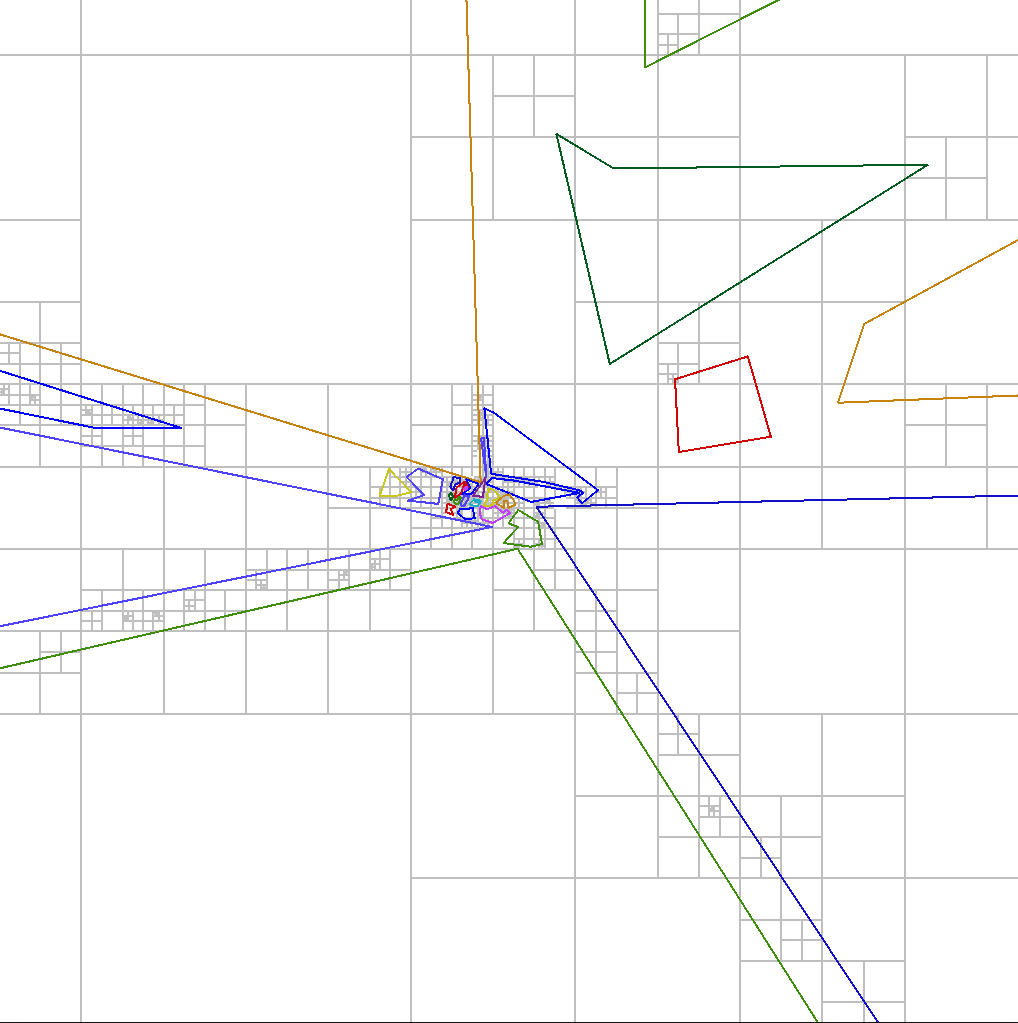
\includegraphics[width=0.31\columnwidth]{ut4.png} }
  \subfloat[][60,000x zoom]{
    \label{fig:ut5}
    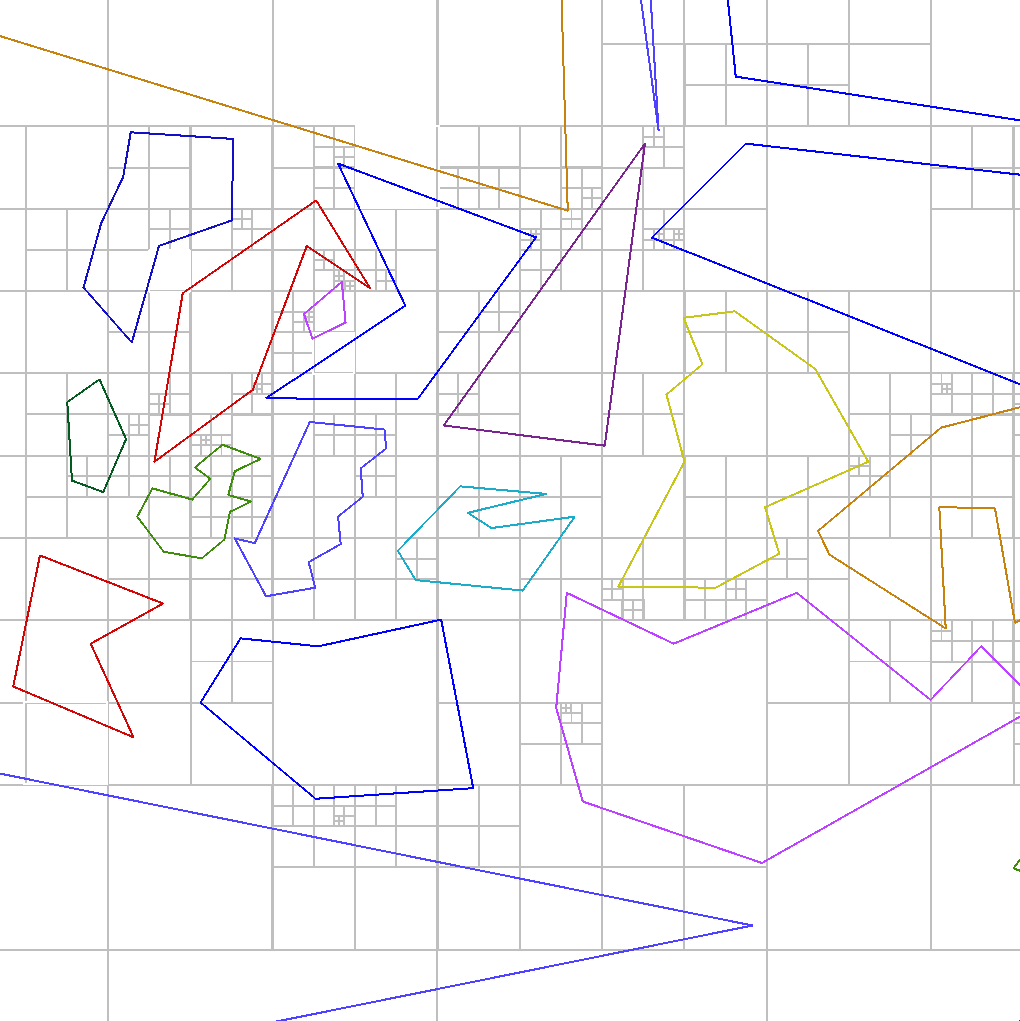
\includegraphics[width=0.31\columnwidth]{ut5.png} }
  \caption{
    \protect\subref{fig:ut1-samples} A complex dataset with 470 objects at vastly different scales in object size and spacing.
    \protect\subref{fig:ut1}-\protect\subref{fig:ut5} Complex dataset at different zoom levels up to 60K magnification. This shows the importance of an adaptive method such as a quadtree. A uniform grid would require $2^{48}$ cells to resolve between objects. The quadtree shown here has $22429$ cells.
  }
  \label{fig:results-maze}
\end{figure}


\begin{figure}
  \centering
  \subfloat[][]{
    \label{fig:gears-1}
    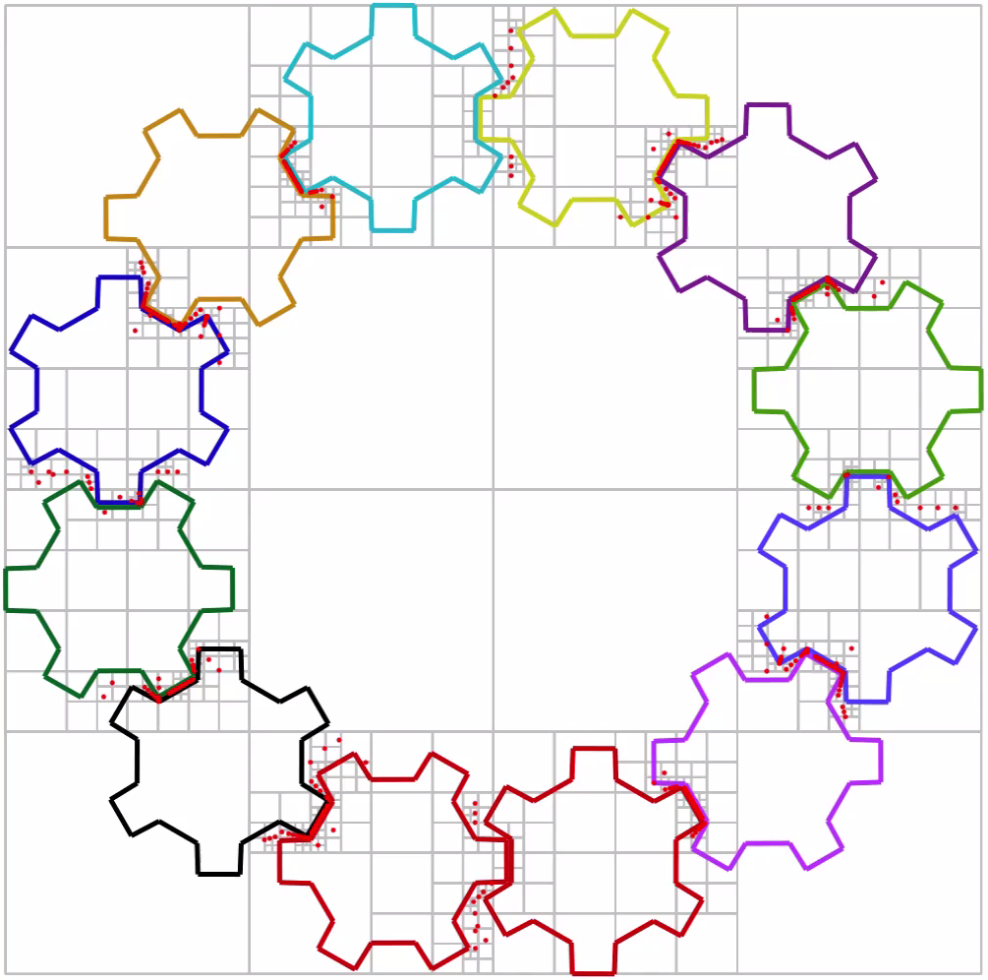
\includegraphics[width=0.31\columnwidth]{Nathan/gears/2.PNG} }
  \subfloat[][]{
    \label{fig:gears-2}
    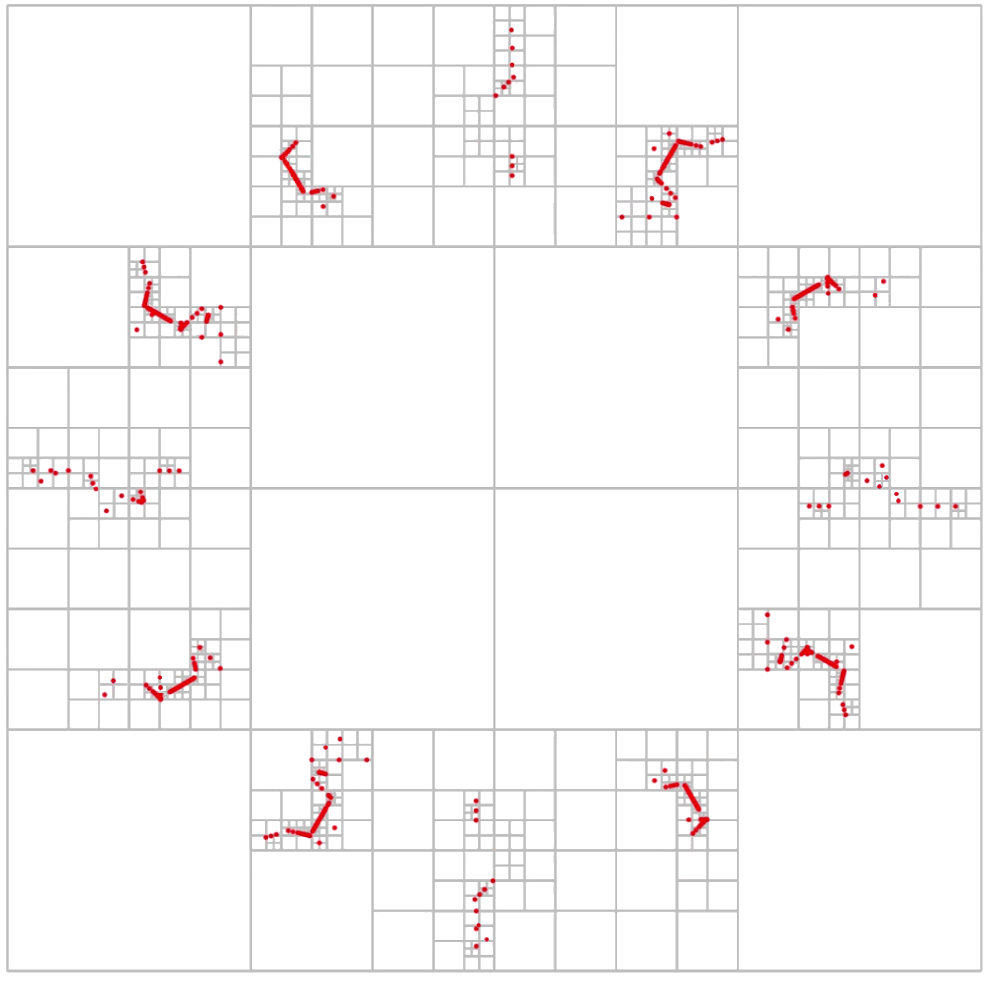
\includegraphics[width=0.31\columnwidth]{Nathan/gears/3.PNG} }
  \subfloat[][]{
    \label{fig:gears-3}
    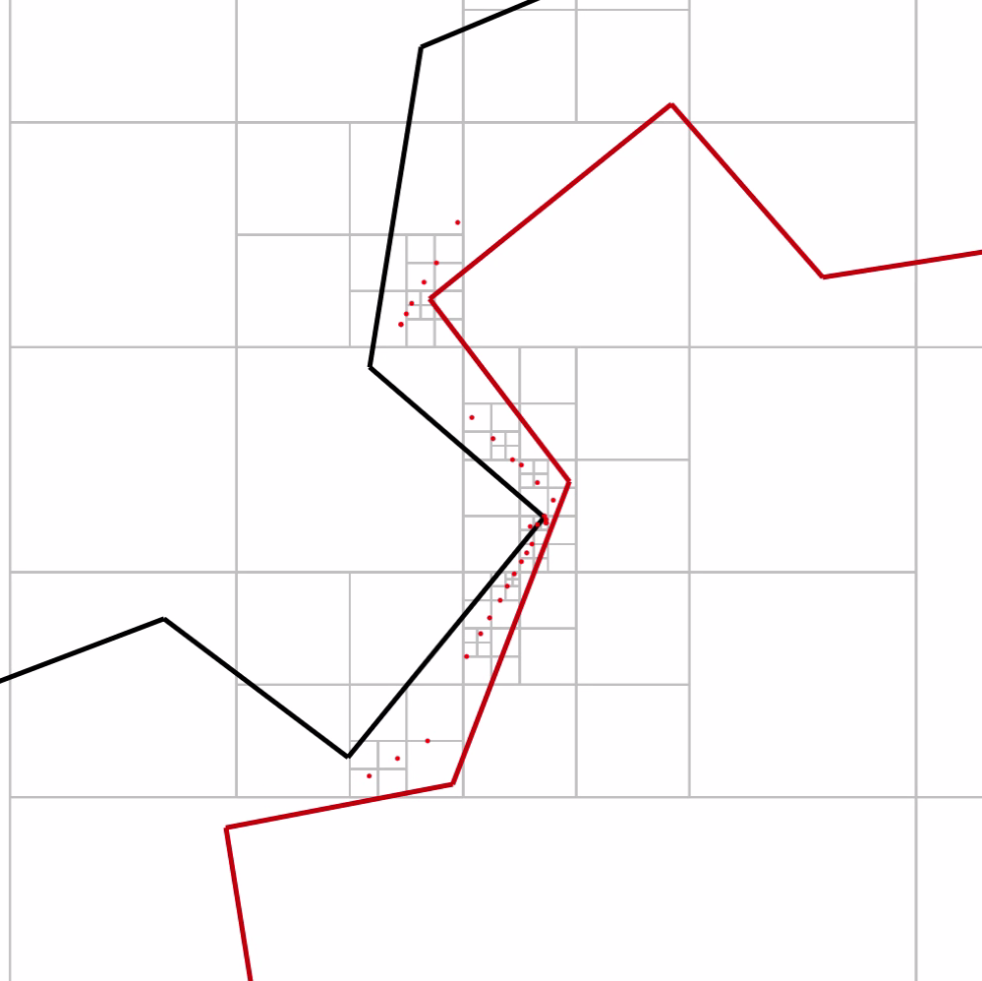
\includegraphics[width=0.31\columnwidth]{Nathan/gears/5.PNG} }
  \caption{
    \protect\subref{fig:gears-1} A dataset of gears with close tolerance. The resolved quadtree with sampled points is shown.
    \protect\subref{fig:gears-2} Showing just the quadtree and sample points.
    \protect\subref{fig:gears-3} A zoomed-in image showing the close object spacing compared to the large domain.
  }
  \label{fig:gears}
\end{figure}

\begin{figure}
  \centering
  \subfloat[][]{
    \label{fig:vascular-1}
    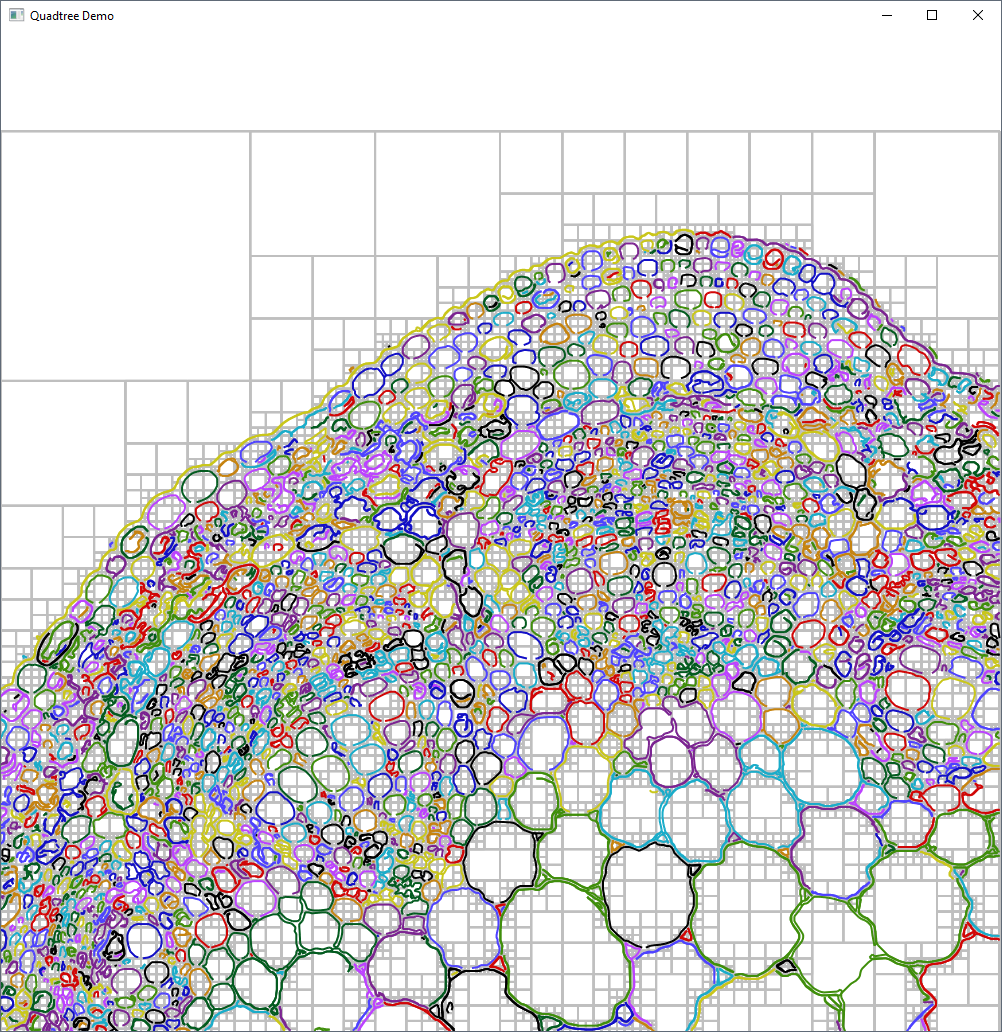
\includegraphics[width=0.31\columnwidth]{Nathan/vascular-bundles/04-Pruned.PNG} }
  \subfloat[][]{
    \label{fig:vascular-2}
    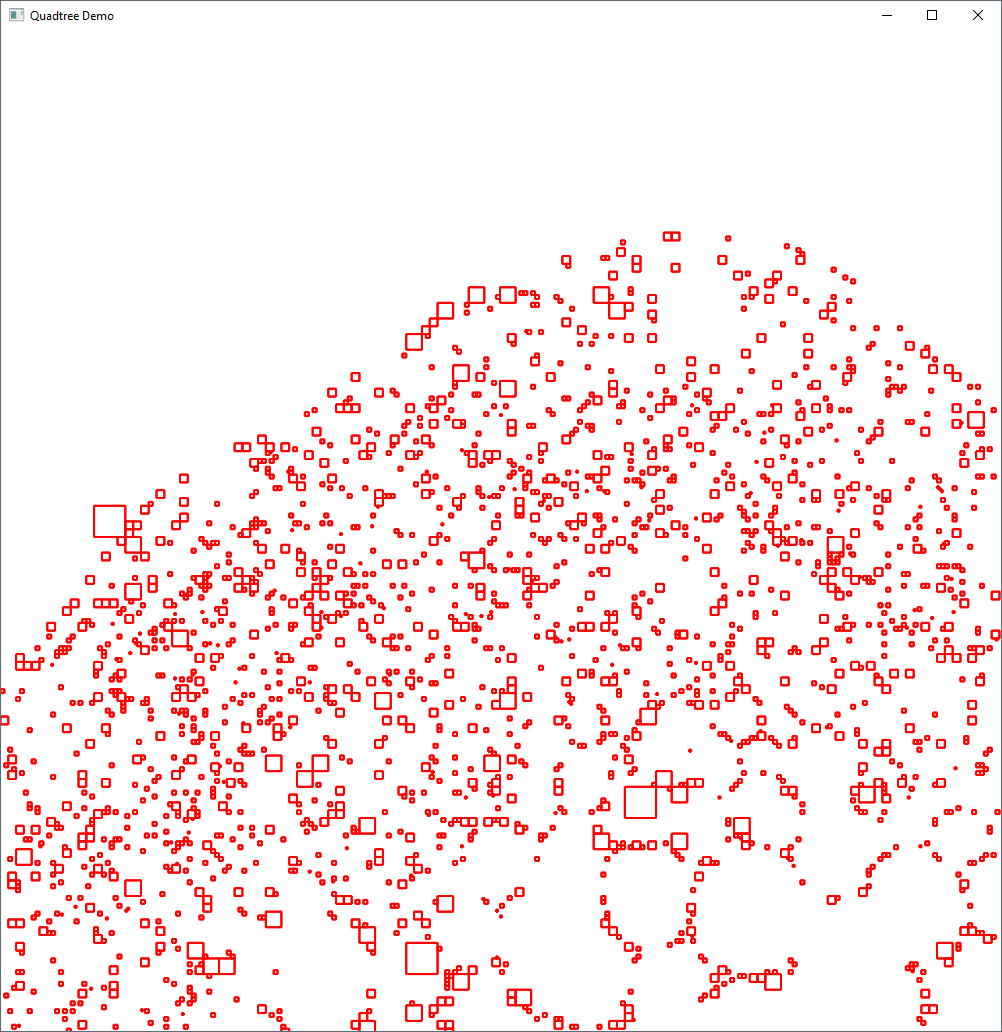
\includegraphics[width=0.31\columnwidth]{Nathan/vascular-bundles/06-Initial-Conflicts.PNG} }
  \subfloat[][]{
    \label{fig:vascular-3}
%    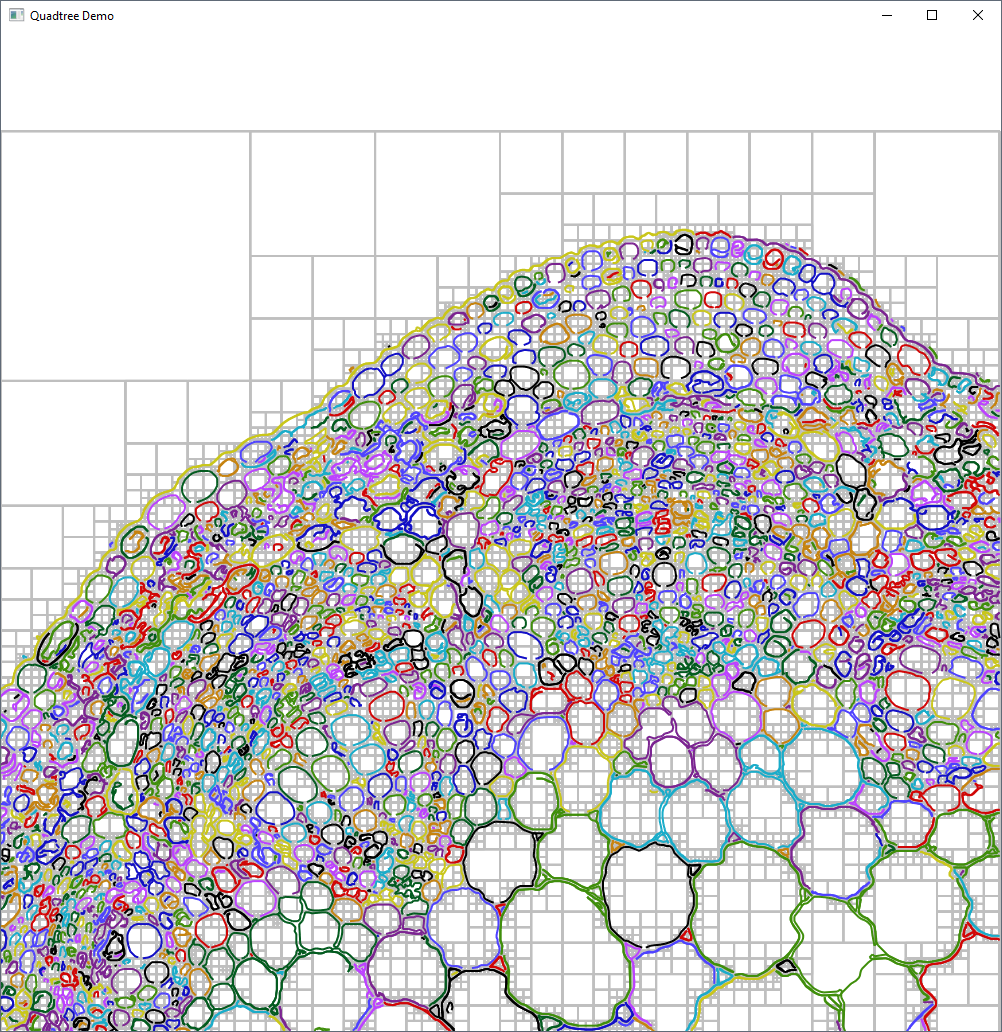
\includegraphics[width=0.31\columnwidth]{Nathan/vascular-bundles/08-Resolved-Quadtree.PNG} }
    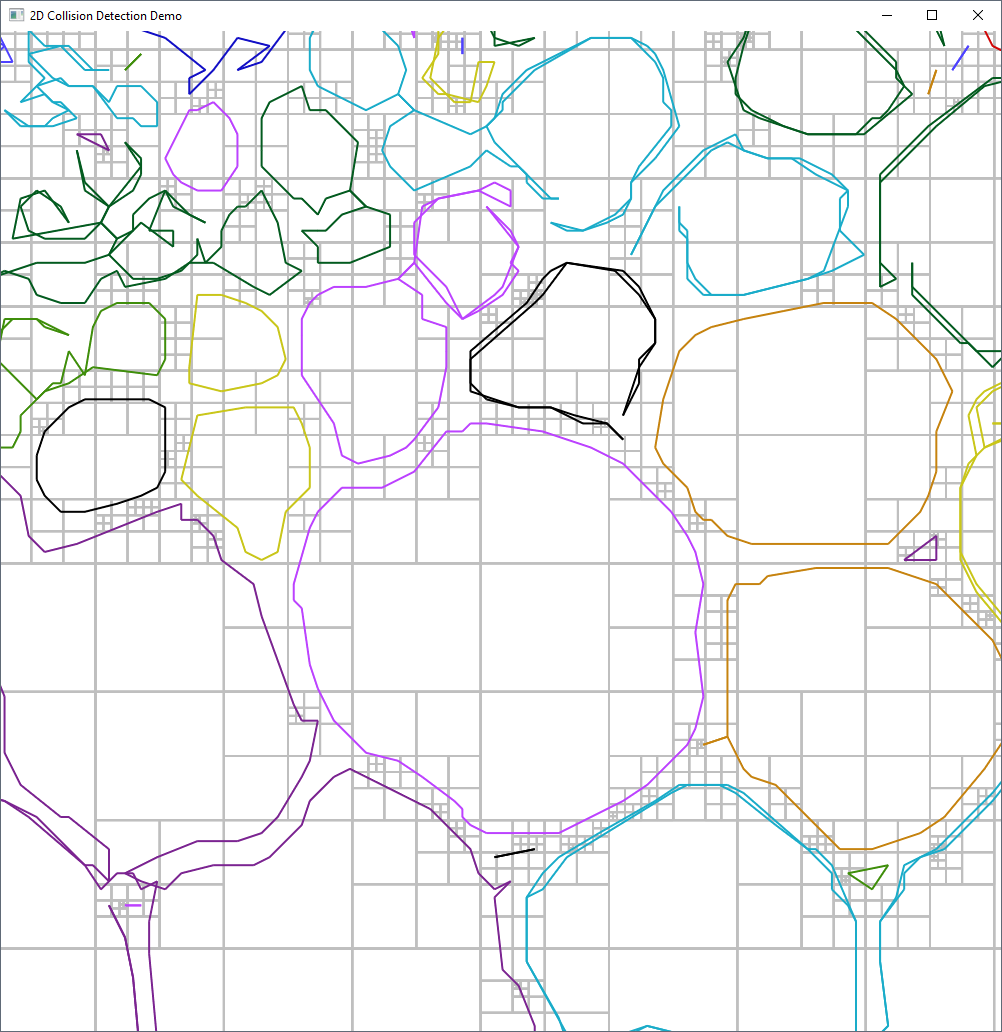
\includegraphics[width=0.31\columnwidth]{Nathan/vascular-bundles/14-Resolved-Quadtree.PNG} }
  \caption{Dataset derived from plant vasculature image.
    \protect\subref{fig:vascular-1} Initial vertex quadtree after pruning.
    \protect\subref{fig:vascular-2} All conflict cells of the initial quadtree.
    \protect\subref{fig:vascular-3} After conflict cell resolution. No quadtree cell intersects more than one object. Our method works even though objects in this dataset are often non-manifold and have self-intersections.
  }
  \label{fig:vascular}
\end{figure}

% # quadtree vertices
%  52K ./viewer3 -l 8 ~/data/gears/gear[1-3].obj
% 170K ./viewer3 -l 12 ~/data/knife/knife-holder.obj ~/data/knife/knife[2-4].obj
% 146K ./viewer2 -l 24 ../data2/filled_ut/*.dat
% 2.8M ./viewer3 --uniform-colors -a 1 -l 8 ~/data/neuron/improved/a*.obj
% 1.3M ./viewer3 -l 8 ~/data/rice-dwarf/decimated2/n1UF2a-*.obj

% memory (54 bytes per quadtree cell)
%  2.8Mb ./viewer3 -l 8 ~/data/gears/gear[1-3].obj
%  9.2Mb ./viewer3 -l 12 ~/data/knife/knife-holder.obj ~/data/knife/knife[2-4].obj
% 7.9Mb ./viewer2 -l 24 ../data2/filled_ut/*.dat
% 151.2Mb ./viewer3 --uniform-colors -a 1 -l 8 ~/data/neuron/improved/a*.obj
% 70.2Mb ./viewer3 -l 8 ~/data/rice-dwarf/decimated2/n1UF2a-*.obj

\begin{table*}
  \centering
  \footnotesize{
%  \begin{tabular}{lcc|cc|cc|cc|cc}
  \begin{tabular}{lcc|cc|cc|cc}
    \toprule
    dataset & objects & object          & \multicolumn{2}{c|}{quadtree}
    & \multicolumn{2}{c|}{time} &  \multicolumn{2}{c}{quad cells} 
    \\
%    & \multicolumn{2}{c}{quad memory}\\
            &         & facets          & \multicolumn{2}{c|}{depth}
    & \multicolumn{2}{c|}{(millisec)} & \multicolumn{2}{c}{($\times 10^3$)}
    \\
%    & \multicolumn{2}{c}{(Mb)}    \\
%            &         & ($\times 10^3$) & Ours & Prev
            &         &  & Ours & Prev
%    & Ours & Prev & Ours & Prev & Ours & Prev \\
    & Ours & Prev & Ours & Prev \\
    %\midrule
    \hline

    % ./gvd-viewer2 -l 9 ../data2/test1*.dat
    % ./QUADTREE --disable-conflict-color -d 1 -m 4 -l 10 data/test1*.dat
    Fig. \ref{fig:simple-conflicts} & 5 & 24 & 10 & 9 & 54 & 3 & 177 & 1168  \\

    % ./gvd-viewer2 -l 24 ../data2/maze/*.dat
    % ./QUADTREE --disable-conflict-color -d 1 -m 3 -l 24 data/maze/poly*.dat
    Fig. \ref{fig:ut1-samples} & 470 & 4943 & 24 & 24 & 128 & 465 & 38 & 157  \\

    % ./gvd-viewer2 -l 8 ../data2/glines/100x100/*.dat
    % ./QUADTREE --disable-conflict-color -d 1 -m 4 -l 9 data/glines/100x100/*
    Fig. \ref{fig:glines} & 2 & 27,998 & 9 & 8 & 148 & 429 & 43 & 66  \\

    % ./gvd-viewer2 -l 9 ../data2/glines/200x200/*.dat
    % ./QUADTREE --disable-conflict-color -d 1 -m 4 -l 10 data/glines/200x200/*
    Fig. \ref{fig:glines} x2 & 2 & 113,084 & 10 & 9 & 414 & 1778 & 125 & 262  \\

    \bottomrule
  \end{tabular}}
  \caption{\red{Nate, please send me an updated table in whatever format (I can throw it into Latex). We should have timings on simple, maze, vascular and gears comparing GVD to PGVD with and without pruning. Not sure if we'll end up including the non-pruning results. We should also include the \# objects, \# facets and \# quadtree cells, as are included in this table.} Table of quadtree computation statistics and timings on datasets that are unmanageable using other methods. Columns are: \emph{objects} - the number of objects in the dataset; \emph{object facets} - the number of line segments (2D) of all objects in the dataset; \emph{quadtree depth} - required quadtree depth in order to resolve objects; \emph{time (ms)} - milliseconds to build the quadtree; \emph{quad cells} - number of quadtree cells. Dataset ``\ref{fig:glines} x2'' is a maze dataset increased in size by a factor of two in each dimension from \ref{fig:glines}. }
  \label{tab:timings}
\end{table*}

As can be seen in table \ref{tab:timings}, there is overhead with our approach: running our algorithm on small datasets yields smaller gains. In fact, our approach actually performs worse on the toy dataset. The power of our algorithm becomes more obvious on large, complex datasets, where our performance time gains are significant.

We are in the process of integrating our algorithm with animated systems, generating quadtrees in real-time for collision detection, distance transforms, and generalized Voronoi diagram computation. Our implementation continues to be refined and optimized, and we expect to shortly have a version with an order of magnitude improvement over the state of the art. Importantly, we are also working on an extension to 3D. Every step in our method has a straightforward extension to 3D with the exception of point sampling for conflict resolution (see section \ref{sec:resolve}), which is where we are focusing our efforts.

%-------------------------------------------------------------------------------
% Conclusions
%-------------------------------------------------------------------------------
%\section{Conclusions}

%-------------------------------------------------------------------------------
% Acknowledgements
%-------------------------------------------------------------------------------
%\section*{Acknowledgements}
%Thanks to Kristen Harris for use of the neuronal data and Jonathan Bronson for the heart data. The work of JE and VP was supported in part by NSF IIS-1314896, NSF ACI-0904631, DOE/NEUP 120341, DOE/UV-CDAT DESC0006872, DOE/Codesign P01180734, DOE/SciDAC DESC0007446, DOE/PIPER DESC0010498, and DOE/CCMSC DENA0002375. This work initiated at the University of Texas when JE, ED  and CB were supported in part by NIH contract R01-EB00487, NSF Grant OCI-1216701 and SNL contract 1439100.

%-------------------------------------------------------------------------
% Bibliography
%-------------------------------------------------------------------------

\bibliographystyle{model3-num-names}
%\bibliographystyle{abbrv}
%\balance
\bibliography{paper}

\end{document}
